\documentclass[bachelor, fontsize=14]{diploma}

\student{Иванов Иван Иванович}
\group{М8О-407Б-19}
\theme{Разработка системы для сравнительного нагрузочного тестирования и визуального анализа производительности реляционных баз данных}

\supervisor{Орлов Марсель Максимович}
\firstConsultant{Алешина Анна Константиновна}
\reviewer{Свиридов Михаил Артемьевич}

\faculty{№ 8 <<Компьютерные науки и прикладная математика>>}
\department{806}
\speciality{01.03.02 <<Прикладная математика и информатика>>}
\profile{Информатика}

\departmentFullName{№ 806}
\headOfDepartment{Крылов Сергей Сергеевич}

% Дата. Оставляем пустое место для дня
\date{\uline{\hspace{24pt}} мая \the\year\ года}

\newacronym{api}{API}{Application Programming Interface — программный интерфейс приложения}
\newacronym{bk}{БД}{база данных}
\newacronym{vkr}{ВКР}{выпускная квалификационная работа}
\newacronym{dbms}{СУБД}{система управления базами данных}
\newacronym{http}{HTTP}{Hypertext Transfer Protocol — протокол передачи гипертекста}
\newacronym{json}{JSON}{JavaScript Object Notation — текстовый формат обмена данными}
\newacronym{orm}{ORM}{Object-Relational Mapping — объектно-реляционное отображение}
\newacronym{rest}{REST}{Representational State Transfer — архитектурный стиль проектирования распределённых систем}
\newacronym{sql}{SQL}{Structured Query Language — язык структурированных запросов}
\newacronym{tps}{TPS}{Transactions Per Second — транзакций в секунду}
\newacronym{ui}{UI}{User Interface — пользовательский интерфейс}
\newacronym{url}{URL}{Uniform Resource Locator — унифицированный указатель ресурса}
\newacronym{ws}{WS}{WebSocket — протокол полнодуплексной связи поверх TCP-соединения}
\newacronym{cpu}{CPU}{Central Processing Unit — центральное процессорное устройство}
\newacronym{ram}{RAM}{Random Access Memory — оперативная память}
\newacronym{io}{I/O}{Input/Output — ввод/вывод}

\newglossaryentry{term1}{
    name={Нагрузочное тестирование},
    description={вид тестирования производительности, направленный на определение поведения системы под ожидаемой и повышенной нагрузкой}
}
\newglossaryentry{term2}{
    name={Система управления базами данных},
    description={программное обеспечение для создания, ведения и управления базами данных, обеспечения доступа к ним и контроля целостности}
}
\newglossaryentry{term3}{
    name={Пропускная способность},
    description={количество успешно обработанных транзакций в единицу времени, измеряемое в TPS (Transactions Per Second)}
}
\newglossaryentry{term4}{
    name={Задержка},
    description={время от отправки запроса к базе данных до получения ответа, измеряемое в миллисекундах}
}
\newglossaryentry{term5}{
    name={Процентиль},
    description={значение, ниже которого находится определённый процент измерений в наборе данных (например, p95 означает, что 95\% запросов выполнены быстрее данного значения)}
}
\newglossaryentry{term6}{
    name={Виртуальный пользователь},
    description={эмулированная сущность, выполняющая транзакции в ходе нагрузочного теста для имитации реальной рабочей нагрузки}
}
\newglossaryentry{term7}{
    name={Сценарий тестирования},
    description={набор параметризованных SQL-запросов с заданным соотношением операций, моделирующих рабочую нагрузку на СУБД}
}
\newglossaryentry{term8}{
    name={Временной ряд},
    description={последовательность значений метрик производительности, зафиксированных через равные интервалы времени в ходе выполнения теста}
}
\newglossaryentry{term9}{
    name={Снапшот состояния},
    description={фиксация состояния базы данных (количество строк в таблицах) перед выполнением теста для последующей верификации целостности}
}
\newglossaryentry{term10}{
    name={Стресс-тестирование},
    description={вид тестирования производительности для определения границ работоспособности системы при экстремальных нагрузках, отличающийся от нагрузочного тестирования}
}
\newglossaryentry{term11}{
    name={Конфигурация сценария нагрузки},
    description={конкретный набор параметризованных SQL-запросов, связанный с профилем схемы и шаблоном сценария; определяет состав, веса и параметры запросов при выполнении тестового прогона}
}
\newglossaryentry{term12}{
    name={Логическая база данных},
    description={именованная группа физических подключений к СУБД, объединённых единым профилем схемы; используется как единица конфигурации при запуске нагрузочного тестирования нескольких экземпляров СУБД}
}
\newglossaryentry{term13}{
    name={Профиль схемы},
    description={описание структуры данных, общей для группы совместимых баз данных одной предметной области; служит основой для автоматической генерации конфигураций сценариев нагрузки}
}
\newglossaryentry{term14}{
    name={Размер эффекта},
    description={стандартизированная мера практической значимости различий между двумя выборками; в настоящей работе применяется коэффициент Коэна~$d$, выражающий величину различия в единицах стандартного отклонения}
}


\addbibresource{main.bib}

\begin{document}
    \maketitle

    % \includepdf[pages=-]{extra/task} % Задание
    \setcounter{page}{2} % Устанавливает счётчик страниц

    \abstract % Структурный элемент: РЕФЕРАТ

\keywords{НАГРУЗОЧНОЕ ТЕСТИРОВАНИЕ, РЕЛЯЦИОННЫЕ БАЗЫ ДАННЫХ, СУБД, ПРОИЗВОДИТЕЛЬНОСТЬ, СРАВНИТЕЛЬНЫЙ АНАЛИЗ, ВЕБ-ИНТЕРФЕЙС, МЕТРИКИ ПРОИЗВОДИТЕЛЬНОСТИ, ВИЗУАЛИЗАЦИЯ}

Объектом исследования являются реляционные системы управления базами данных и их поведение под контролируемой нагрузкой. Предметом исследования выступают методы, алгоритмы и инструментальные средства для автоматизированного нагрузочного тестирования, сбора метрик производительности и визуализации результатов с целью сравнительного анализа. Объектом разработки является программный комплекс для сравнительного нагрузочного тестирования реляционных СУБД. Цель работы~--- создание инструмента, обеспечивающего автоматизированное тестирование, сбор метрик производительности и их анализ через единый веб-интерфейс.

В работе применены методы системного и объектно-ориентированного проектирования, математической статистики для сопоставления прогонов и экспериментального исследования производительности СУБД. Разработана клиент-серверная система с веб-интерфейсом и поддержкой MySQL, PostgreSQL и MariaDB; реализованы формирование нагрузки по сценариям, отображение метрик в реальном времени, хранение истории прогонов, сравнительный анализ результатов, а также подготовка и восстановление состояния баз данных при тестах с операциями записи. Развёртывание системы выполняется средствами Docker Compose.

Работоспособность подтверждена экспериментально на двух наборах данных~--- Sakila и Brazilian E-Commerce~--- при сравнении трёх СУБД; проведено 12~прогонов с нулевой долей ошибок.

Практическая значимость работы заключается в том, что результаты тестирования можно использовать для сравнения СУБД, оценки ускорения после изменений и выявления снижения производительности. % Реферат

    \tableofcontents % Содержание 
    \termsanddefenitions % Термины и определения
    \listofabbreviations % Перечень сокращений и обозначений
 
    \introduction % Структурный элемент: ВВЕДЕНИЕ

В современном цифровом мире, где данные стали одним из ключевых активов, эффективность их обработки и хранения напрямую определяет успешность бизнес-процессов, качество пользовательского опыта и, в конечном счёте, финансовые результаты организаций. Основой большинства информационных систем остаются системы управления базами данных, от производительности которых зависит скорость отклика приложений, стабильность работы под нагрузкой и возможность масштабирования. Особую значимость эти вопросы приобретают в контексте постоянного роста объёмов данных, усложнения запросов и повышения требований к доступности сервисов.

Однако существующие инструменты для нагрузочного тестирования баз данных зачастую не предоставляют комплексного решения. Многие из них требуют глубоких технических знаний для настройки, проводят тестирование в изолированной среде без возможности простого сопоставления результатов нескольких прогонов, а их выводы ограничиваются текстовыми отчётами или сырыми данными, требующими трудоемкой ручной обработки и анализа. Отсутствие интегрированной платформы, которая бы автоматизировала процесс тестирования, обеспечивала наглядную визуализацию ключевых метрик в реальном времени и позволяла проводить удобное сравнительное исследование, создаёт существенный барьер для оперативной диагностики узких мест и обоснованного принятия решений по оптимизации. В связи с этой проблемой становится актуальной разработка программного комплекса, который заполнит указанный пробел.

Целью данной выпускной квалификационной работы является разработка и внедрение программного комплекса, позволяющего в автоматическом режиме проводить нагрузочное тестирование реляционных СУБД, собирать ключевые метрики производительности и предоставлять результаты в наглядном виде через единый веб-интерфейс для последующего анализа и сравнения.

Для достижения поставленной цели необходимо решить следующие задачи:
\begin{enumerate}[label=\arabic*)]
    \item провести анализ современных подходов к нагрузочному тестированию СУБД и сформулировать требования к разрабатываемой системе;
    \item разработать и реализовать ядро системы для автоматизированного тестирования производительности с поддержкой SQL-сценариев и транзакционной нагрузки;
    \item спроектировать и создать веб-интерфейс для управления процессом тестирования и визуального анализа результатов;
    \item выполнить комплексное тестирование системы на тестовых стендах и проанализировать полученные результаты.
\end{enumerate}

Объектом исследования выступают реляционные системы управления базами данных и их поведение под контролируемой нагрузкой. Предметом исследования являются методы, алгоритмы и инструментальные средства для автоматизированного проведения нагрузочного тестирования, сбора метрик производительности и визуализации результатов с целью сравнительного анализа.

В работе применяются методы системного анализа для проектирования архитектуры, методы объектно-ориентированного проектирования для реализации модулей системы, методы математической статистики для сравнительного анализа результатов тестирования, а также методы экспериментального исследования для оценки производительности СУБД.

Практическая значимость работы заключается в создании инструмента, который позволяет не только измерять, но и наглядно сравнивать производительность различных СУБД, что является основой для обоснованного выбора технологий, оценки эффективности оптимизаций и предотвращения регрессии после внесения изменений. Целевой аудиторией системы являются инженеры по производительности, DevOps-инженеры, администраторы баз данных и разработчики.

Структура работы включает введение, четыре главы, заключение и список использованных источников. В первой главе проводится аналитический обзор существующих решений и формулируются требования. Во второй главе описывается проектирование архитектуры и модулей системы. В третьей главе рассматривается программная реализация. В четвёртой главе представлены результаты экспериментального тестирования~--- двенадцать прогонов~--- и анализ производительности на двух тестовых наборах данных. % Введение

    \section{АНАЛИТИЧЕСКАЯ ЧАСТЬ}

\subsection{Нагрузочное тестирование СУБД: понятия, цели, методологии}

Производительность баз данных является одним из определяющих факторов качества современных информационных систем. С ростом объёмов обрабатываемых данных и увеличением числа одновременных пользователей задача объективной оценки производительности СУБД приобретает критическое значение. Нагрузочное тестирование представляет собой основной метод её решения, позволяя определить поведение системы под контролируемой нагрузкой и выявить потенциальные узкие места до их проявления в промышленной эксплуатации~\cite{gregg_2020}.

Нагрузочным тестированием называется вид тестирования производительности, направленный на определение поведения системы при ожидаемой и повышенной нагрузке, создаваемой путём эмуляции работы множества одновременных пользователей. Важно разграничивать нагрузочное тестирование и стресс-тестирование: первое оценивает работу системы в рамках проектных параметров нагрузки, второе определяет границы работоспособности при экстремальных значениях, превышающих нормальные эксплуатационные характеристики. Отдельным видом является тестирование стабильности , при котором система подвергается длительной нагрузке для выявления деградации производительности, утечек памяти и накопления фрагментации данных. Совместное применение указанных видов тестирования позволяет получить полную картину поведения СУБД в различных нагрузочных сценариях.

Ключевыми метриками, измеряемыми в процессе нагрузочного тестирования СУБД, являются задержка и пропускная способность~\cite{kleppmann_2017}. Задержка характеризует время от отправки запроса к базе данных до получения ответа и измеряется в миллисекундах. Для полного описания распределения задержек применяются процентили: медиана (p50) отражает типичное время отклика, p95 показывает задержку, которую не превышают 95\,\% запросов, а p99 характеризует наихудшие случаи. Использование исключительно среднего значения задержки является недостаточным, поскольку оно маскирует выбросы, способные существенно влиять на пользовательский опыт. Пропускная способность измеряется количеством успешно обработанных единиц нагрузки в секунду: запросов для SQL-сценариев и транзакций для транзакционных сценариев. Зависимость между задержкой и пропускной способностью нелинейна: при достижении определённого порога нагрузки пропускная способность перестаёт расти, а задержка начинает экспоненциально увеличиваться. Точка, в которой пропускная способность достигает максимума, называется точкой насыщения и является важным параметром при определении предельной нагрузки на систему.

Помимо основных метрик, в процессе тестирования отслеживаются системные показатели: загрузка центрального процессора, использование оперативной памяти, интенсивность дискового ввода-вывода. Из внутренних показателей СУБД особый интерес представляют коэффициент попаданий в кэш и количество взаимных блокировок. Коэффициент попаданий в кэш отражает долю запросов, обработанных без обращения к диску, и служит индикатором эффективности использования буферного пула. Взаимные блокировки возникают при конкурентном доступе к данным и приводят к принудительному завершению части транзакций, снижая общую пропускную способность. Рост частоты блокировок при увеличении числа параллельных транзакций сигнализирует о необходимости оптимизации структуры запросов или уровня изоляции транзакций.

Стандартизацией методологий тестирования производительности СУБД занимается организация TPC~--- всемирный консорциум, устанавливающий стандарты для оценки быстродействия и надёжности систем обработки транзакций и баз данных~\cite{tpc_specs}. Наиболее значимыми спецификациями TPC для реляционных СУБД являются TPC-C, TPC-H и TPC-E.

Спецификация TPC-C моделирует среду обработки заказов, в которой множество пользователей одновременно выполняют транзакции нескольких типов: оформление заказов, регистрация платежей, проверка статусов и мониторинг складских запасов. Бенчмарк охватывает пять типов параллельных транзакций различной сложности, обеспечивая комплексную проверку компонентов СУБД. Основной метрикой TPC-C является количество новых заказов в минуту~--- tpmC. Данная спецификация широко применяется для оценки OLTP-систем и реализована в ряде инструментов тестирования, в частности в HammerDB под наименованием TPROC-C. Спецификация TPC-H ориентирована на системы поддержки принятия решений и представляет собой набор бизнес-ориентированных ad-hoc запросов и модификаций данных; её основная метрика~--- составной показатель производительности запросов в час QphH@Size; в инструментах тестирования данная нагрузка фигурирует под наименованием TPROC-H. Спецификация TPC-E представляет более современную OLTP-модель, воспроизводящую деятельность брокерской фирмы с асинхронными операциями и сложным профилем чтения и записи; метрика~--- количество транзакций в секунду. По сравнению с TPC-C, TPC-E обеспечивает более реалистичную нагрузку для современных онлайн-систем.

Параллельно с автоматизацией тестирования сформировалась концепция наблюдаемости, объединяющая сбор, хранение и анализ телеметрических данных в режиме реального времени. Ключевым компонентом такого стека в области мониторинга метрик является система Prometheus~--- открытое программное обеспечение для сбора и хранения временных рядов с многомерной моделью данных~\cite{prometheus_overview}. Данные в Prometheus идентифицируются по имени метрики и набору меток в формате ключ--значение, что позволяет выполнять гибкую фильтрацию и агрегацию с помощью языка запросов PromQL. Для унификации инструментирования приложений разработан стандарт OpenTelemetry~--- независимый от поставщика фреймворк, охватывающий трассировки, метрики и журналы и обеспечивающий передачу телеметрии через единый компонент OpenTelemetry Collector в различные бэкенды~\cite{opentelemetry}. Совместное применение Prometheus и OpenTelemetry формирует полноценный стек наблюдаемости, позволяющий коррелировать результаты нагрузочных тестов с системными показателями. Необходимо отметить, что организация TPC расширяет область стандартизации за рамки реляционных СУБД: в частности, спецификация TPCx-AI адресована платформам машинного обучения и аналитики данных, однако данное направление выходит за рамки предметной области настоящей работы.

Типовая методология нагрузочного тестирования СУБД включает несколько последовательных этапов. На этапе подготовки определяется цель тестирования, выбирается или формируется тестовая база данных, создаются сценарии нагрузки и настраивается тестовый стенд. На этапе прогрева  система выводится на стабильный режим работы, исключающий влияние начальной инициализации кэшей и буферов. Основной этап заключается в выполнении нагрузки с заданным числом виртуальных пользователей и фиксацией метрик через равные интервалы времени. Завершающий этап анализа предполагает вычисление агрегированных показателей, построение зависимостей метрик от нагрузки и формулировку выводов.

Таким образом, нагрузочное тестирование СУБД представляет собой комплексный процесс, охватывающий определение целей, выбор методологии, генерацию контролируемой нагрузки, сбор и анализ метрик производительности. Стандартизированные спецификации TPC обеспечивают сопоставимость результатов между различными системами. Рассмотренные методологии и метрики составляют теоретическую основу для анализа существующих инструментальных решений, представленного в следующем разделе.

\subsection{Обзор существующих инструментов}

Прежде чем анализировать конкретные инструменты, необходимо определить критерии их отбора и логику классификации. В рамках настоящего обзора рассматриваются решения, непосредственно применимые к нагрузочному тестированию реляционных СУБД: инструменты должны поддерживать хотя бы одну из целевых СУБД, генерировать контролируемую нагрузку и собирать метрики производительности. По характеру своего происхождения и целевой аудитории все рассматриваемые решения разбиваются на три группы: классические инструменты для реляционных СУБД с открытым исходным кодом, современный DevOps-ориентированный инструментарий и коммерческие корпоративные решения. Такая классификация позволяет выявить не просто отдельные достоинства и недостатки продуктов, но закономерности, характерные для каждого класса в целом.

\subsubsection{Классические инструменты для реляционных СУБД}

Sysbench~--- кроссплатформенный инструмент нагрузочного тестирования и бенчмаркинга с открытым исходным кодом, изначально созданный для MySQL и впоследствии расширенный поддержкой PostgreSQL. Инструмент предоставляет набор встроенных OLTP-сценариев, охватывающих операции чтения, записи, обновления и удаления данных, и допускает создание пользовательских сценариев на языке Lua, что обеспечивает значительную гибкость конфигурирования. Ключевые метрики выходного отчёта~--- количество транзакций в секунду и время отклика. Основным достоинством Sysbench является сочетание простоты установки с широкими возможностями параметризации через Lua-скрипты. Вместе с тем инструмент ограничен интерфейсом командной строки, лишён механизмов хранения истории тестов и не предусматривает автоматизированного сравнения результатов между прогонами, что вынуждает пользователя самостоятельно интерпретировать и сопоставлять текстовые отчёты.

Утилита pgbench входит в стандартную поставку PostgreSQL и моделирует банковскую транзакционную нагрузку по мотивам спецификации TPC-B, измеряя количество транзакций в секунду при заданном числе параллельных клиентских соединений. Инструмент поддерживает выполнение пользовательских SQL-скриптов, что несколько расширяет область его применения за пределы встроенного бенчмарка. Главное достоинство pgbench состоит в отсутствии необходимости установки дополнительного программного обеспечения для пользователей PostgreSQL. Однако жёсткая привязка к одной СУБД, упрощённая модель нагрузки и минимальные возможности визуализации существенно сужают сферу применимости инструмента и делают его скорее отправной точкой для экспресс-оценки, нежели полноценным средством сравнительного анализа производительности.

HammerDB~--- инструмент нагрузочного тестирования и бенчмаркинга баз данных с открытым исходным кодом, разрабатываемый под эгидой организации TPC. Актуальная версия 5.0 распространяется под лицензией GNU GPL v3.0~\cite{hammerdb_v5}. В данном выпуске HammerDB перешёл на бинарные дистрибутивы в виде единых исполняемых файлов для трёх режимов работы: графический интерфейс, интерфейс командной строки и веб-сервис. Ядро инструмента переработано на базе Tcl/Tk\,9.0~--- первого крупного обновления за более чем 27 лет. HammerDB поддерживает MariaDB, PostgreSQL, Oracle, SQL Server, MySQL и IBM\,Db2. Инструмент реализует рабочие нагрузки TPROC-C и TPROC-H~--- производные от спецификаций TPC-C и TPC-H~--- с результирующими метриками NOPM (New Orders Per Minute) и TPM (Transactions Per Minute). Ключевым преимуществом HammerDB является широкая поддержка СУБД в сочетании с соответствием отраслевым стандартам и доступностью официальных образов Docker для интеграции в CI/CD-окружения. Существенным ограничением остаётся отсутствие централизованного механизма хранения истории тестов: каждый прогон представляет собой изолированное событие, а отслеживание динамики изменений производительности возлагается на пользователя. Таким образом, HammerDB закрывает задачу генерации стандартизированной нагрузки, но не решает задачу долгосрочного сравнительного анализа результатов.

\subsubsection{Коммерческие корпоративные решения}

Benchmark Factory 9.1 ~--- коммерческий инструмент тестирования производительности баз данных, позиционируемый как многоплатформенное решение для корпоративного сегмента~\cite{benchmarkfactory_91}. Benchmark Factory позволяет проводить воспроизведение рабочей нагрузки, отраслевые стандартизированные бенчмарки и тестирование масштабируемости. Инструмент доступен для Oracle, SQL Server, IBM DB2, SAP, MySQL, PostgreSQL, MariaDB и других баз данных через ODBC-подключение. Результаты тестирования сохраняются в централизованном репозитории с поддержкой встроенных отчётов и возможностью просмотра нескольких прогонов одновременно; предусмотрен REST API для автоматизации. Ключевое преимущество Benchmark Factory по сравнению с инструментами класса Oracle RAT~--- поддержка нескольких СУБД в рамках единого продукта с GUI. Вместе с тем инструмент является платным решением с графическим интерфейсом настольного приложения, что ограничивает его доступность для академических и небольших проектов и исключает нативный веб-доступ.

Oracle Real Application Testing~--- коммерческий инструмент корпорации Oracle для тестирования производительности баз данных Oracle, доступный исключительно в составе редакции Oracle Enterprise Edition. Компонент Database Replay позволяет зафиксировать реальную рабочую нагрузку продуктивной базы данных и воспроизвести её на тестовой системе, а компонент SQL Performance Analyzer оценивает влияние изменений на выполнение отдельных SQL-запросов, сравнивая планы выполнения и метрики до и после изменений. Несмотря на высокую точность воспроизведения реальной нагрузки, Oracle RAT жёстко привязан к экосистеме Oracle и требует существенных лицензионных затрат, что принципиально ограничивает его применимость в контексте сравнительного тестирования нескольких СУБД.

\subsubsection{Воспроизводимость бенчмаркинга как концептуальный ориентир}

Отдельного упоминания заслуживает инструмент Benchkit~--- открытый фреймворк, решающий не задачу генерации нагрузки, а задачу воспроизводимости бенчмаркинга: декларативное описание окружения, фиксация всех параметров и результатов теста, автоматизация повторных запусков~\cite{benchkit_exasol}. Данная концепция воспроизводимых конвейеров тестирования представляет интерес с точки зрения проектирования системы централизованного хранения и сравнения истории тестов.

Проведённый обзор позволяет констатировать: каждый из рассмотренных инструментов эффективно решает одну конкретную задачу~--- генерацию нагрузки или анализ производительности~--- но ни одно открытое решение не объединяет в едином интерфейсе генерацию нагрузки на реляционные СУБД, мониторинг метрик в реальном времени, централизованное хранение истории тестов и автоматизированное сравнение прогонов. Описанная фрагментированность служит предметом систематического сравнительного анализа в следующем разделе.

\subsection{Сравнительный анализ решений}

Для систематизации результатов обзора проведён сравнительный анализ рассмотренных инструментов по критериям, непосредственно влияющим на удобство и эффективность практики нагрузочного тестирования СУБД. Выбор критериев обусловлен не техническими характеристиками самих инструментов, а практическими требованиями к процессу сравнительного тестирования нескольких СУБД. Пользовательский интерфейс рассматривается как критерий доступности: CLI-инструменты требуют технической экспертизы и не позволяют наблюдать динамику метрик в реальном времени, тогда как браузерный интерфейс снижает порог входа и обеспечивает немедленную визуальную обратную связь без установки дополнительного программного обеспечения. Наличие истории тестов оценивается как критически важная характеристика: разовый прогон фиксирует состояние системы в единственный момент времени, тогда как только накопленная история позволяет выявлять регрессии производительности и долгосрочные тренды после изменений конфигурации или схемы данных. Возможность сравнения результатов производна от наличия истории и определяет, насколько процесс вынесения суждений о производительности автоматизирован, а насколько возложен на пользователя. Результаты анализа сведены в таблицу~\ref{tab:comparison}.

{
\renewcommand{\arraystretch}{0.9}
\setlength{\tabcolsep}{3pt}
\sloppy
\pretolerance=10000
\tolerance=2000
\emergencystretch=1em
\hyphenpenalty=50
\exhyphenpenalty=50

\begin{table}[H]
    \centering
    \caption{Сравнительный анализ инструментов нагрузочного тестирования СУБД}
    \label{tab:comparison}
    \begin{tabularx}{\textwidth}{|>{\RaggedRight}p{0.13\textwidth}|>{\RaggedRight}X|>{\RaggedRight}X|>{\RaggedRight}X|>{\RaggedRight}X|}
        \hline
        Критерий & HammerDB 5.0 & Sysbench / pgbench & Oracle RAT & Benchmark Factory 9.1 \\
        \hline
        Интер\-фейс & GUI\slash CLI\slash Web & CLI & GUI\slash CLI & GUI\slash CLI\slash REST API \\
        \hline
        Под\-дер\-жи\-ва\-емые СУБД & Oracle, SQL Server, Db2, MySQL, MariaDB, PostgreSQL & MySQL, PostgreSQL (pgbench~--- только PostgreSQL) & Только Oracle Database & Oracle, SQL Server, Db2, MySQL, PostgreSQL, SAP, MariaDB и др. \\
        \hline
        Хранение истории тестов & Отсутствует (логи) & Отсутствует & Частично & Цент\-ра\-ли\-зо\-ван\-ный репо\-зи\-то\-рий \\
        \hline
        Сравнение тестов & Ручной анализ логов & Ручное & Встроенное & Встроенные отчёты \\
        \hline
        Ви\-зу\-а\-ли\-за\-ция & Простые графики & Текстовый отчёт & Детальные отчёты OEM & Встроенные отчёты \\
        \hline
        Модель рас\-про\-стра\-не\-ния & Открытая & Открытая & Прo\-прие\-тар\-ная & Прo\-прие\-тар\-ная \\
        \hline
    \end{tabularx}
\end{table}
}

Анализ таблицы~\ref{tab:comparison} выявляет устойчивые закономерности, характерные для каждого класса инструментов, которые не сводятся к отдельным достоинствам и недостаткам конкретных продуктов.

Инструменты с открытым исходным кодом~--- HammerDB, Sysbench и pgbench~--- демонстрируют общий паттерн: высокая гибкость в части генерации нагрузки при принципиальном отсутствии механизмов долгосрочного накопления и сравнения результатов. Каждый прогон существует как изолированный артефакт; сопоставление результатов между прогонами остаётся ручной операцией, полностью возлагаемой на пользователя. Такая архитектура оправдана для разовых замеров производительности, однако делает перечисленные инструменты непригодными для систематического отслеживания изменений производительности во времени без создания вспомогательной инфраструктуры хранения и анализа данных.

Коммерческие продукты~--- Oracle RAT и Benchmark Factory 9.1~--- предлагают наиболее развитый функционал в части анализа: централизованные репозитории результатов, встроенные сравнительные отчёты, поддержку нескольких типов рабочей нагрузки. Однако данный класс инструментов ограничен по-разному: Oracle RAT жёстко привязан к экосистеме одного поставщика и недоступен вне Oracle Enterprise Edition, тогда как Benchmark Factory, при широте поддерживаемых СУБД, является платным продуктом с настольным графическим интерфейсом, что исключает нативный веб-доступ и существенно ограничивает применимость в академических и некоммерческих проектах.

Таким образом, рассмотренные инструменты образуют фрагментированную экосистему, в которой ни одно решение с открытым исходным кодом не обеспечивает одновременно генерацию нагрузки на несколько реляционных СУБД, мониторинг метрик в реальном времени через браузерный интерфейс, централизованное хранение истории тестов и автоматизированное сравнение прогонов. Коммерческие продукты частично закрывают этот разрыв, однако за счёт закрытости экосистемы или высокой стоимости лицензирования. Выявленный функциональный разрыв определяет состав требований к разрабатываемой системе, сформулированных в следующем разделе.

\subsection{Требования к разрабатываемой системе}

На основании проведённого аналитического обзора и систематического выявления структурных недостатков существующих решений сформулированы требования к разрабатываемой системе сравнительного нагрузочного тестирования реляционных СУБД. Требования разделены на функциональные, нефункциональные и ограничения; каждое из них непосредственно вытекает из функционального разрыва, зафиксированного в разделе~1.3.

Функциональные требования определяют действия, которые система обязана выполнять. Система должна обеспечивать поддержку трёх реляционных СУБД~--- MySQL, MariaDB и PostgreSQL~--- с возможностью сохранения нескольких конфигураций подключений и их совместного использования в рамках одного тестового прогона. Данное требование вытекает из необходимости обеспечить единую точку управления разнородными СУБД, что является ключевым пробелом существующих открытых инструментов.

Система должна поддерживать объединение нескольких физических подключений с одинаковой структурой данных в группу и автоматически подбирать к ней подходящий набор сценариев нагрузки, что позволяет проводить сравнительное тестирование без ручного конфигурирования каждого подключения. Генерация нагрузки должна осуществляться по параметризованным сценариям, которые задают состав операций~--- как отдельных SQL-запросов, так и последовательностей операций в рамках атомарных транзакций~--- с настраиваемым соотношением типов, числом виртуальных пользователей, числом итераций и длительностью прогрева.

Система должна обеспечивать потоковую передачу метрик производительности в веб-интерфейс с задержкой не более одной секунды и параллельно сохранять историю прогонов с возможностью фильтрации и просмотра ранее выполненных тестов. Система должна предоставлять инструменты сравнительного анализа двух и более прогонов~--- как попарного сравнения СУБД при одинаковой нагрузке, так и анализа изменения характеристик при последовательном увеличении числа виртуальных пользователей~--- с автоматическим применением статистических критериев, вычислением размера эффекта и формированием структурированного отчёта.

Система должна автоматически сохранять состояние тестируемых баз данных перед прогонами, включающими операции записи, и восстанавливать его по завершении теста с верификацией целостности данных, что обеспечивает воспроизводимость экспериментов.

Нефункциональные требования определяют качественные характеристики системы. Веб-интерфейс должен быть доступен через стандартный браузер без установки дополнительного программного обеспечения на стороне клиента~--- в противовес настольным GUI-решениям, характерным для коммерческого сегмента. Архитектура системы должна допускать расширение перечня поддерживаемых СУБД без значительной модификации кодовой базы, обеспечивая открытость к развитию. Развёртывание должно осуществляться с использованием контейнеризации, что гарантирует воспроизводимость тестового окружения и упрощает установку в различных инфраструктурах.

Ограничения фиксируют рамки применимости системы в текущей версии. Система предназначена для сравнительного анализа производительности, а не для проведения формальных сертифицированных бенчмарков TPC. Генерация нагрузки осуществляется на одном сервере; горизонтальное масштабирование генераторов нагрузки в текущей версии не предусматривается. Область применения системы ограничена реляционными СУБД.

Сформулированные требования определяют функциональные и технические характеристики разрабатываемой системы и составляют непосредственную основу для проектирования её архитектуры, рассматриваемого во второй главе.

\subsection{Выводы по главе}

Анализ существующих инструментов нагрузочного тестирования показал, что ни одно открытое решение не сочетает генерацию нагрузки на несколько СУБД, мониторинг метрик в реальном времени через браузер, централизованное хранение истории тестов и автоматизированный сравнительный анализ со статистикой. Выявленный пробел позволил сформулировать восемь функциональных требований (включая поддержку трёх СУБД в едином интерфейсе, группы подключений, параметризованные сценарии, потоковую передачу метрик, историю прогонов, двухрежимный анализ и автоматическое резервное копирование), а также нефункциональные требования и ограничения. % Глава 1. Аналитическая часть
    \section{ПРОЕКТИРОВАНИЕ СИСТЕМЫ}

\subsection{Архитектура системы}

Разрабатываемая система построена по многоуровневой клиент-серверной архитектуре с разделением на серверную и клиентскую части. Серверная часть реализована на языке Python с использованием фреймворка FastAPI и обеспечивает генерацию нагрузки, сбор метрик, управление подключениями к тестируемым СУБД, хранение истории тестов, а также управление профилями схем и логическими базами данных. Клиентская часть реализована на TypeScript с использованием фреймворка Next.js и предоставляет веб-интерфейс для управления тестированием, визуализации метрик в реальном времени и анализа результатов.

Взаимодействие между клиентской и серверной частями осуществляется по двум каналам. REST API используется для выполнения CRUD-операций с тестами, сценариями, подключениями, логическими базами данных и профилями схем, а также для запуска тестов и получения результатов. WebSocket обеспечивает двустороннюю связь для трансляции метрик производительности в реальном времени в ходе выполнения теста. Такая архитектура позволяет клиенту инициировать тестирование через HTTP-запрос и затем наблюдать за его ходом через WebSocket-соединение без необходимости периодического опроса сервера.

В процессе работы система взаимодействует с СУБД двух принципиально разных типов. Собственная СУБД системы~--- PostgreSQL~15, хранящая базу данных \texttt{project\_data},~--- предназначена для хранения истории тестов, конфигураций сценариев нагрузки, конфигураций подключений и результатов анализа. Вторая группа~--- целевые базы данных, работающие под управлением СУБД (PostgreSQL, MySQL, MariaDB), над которыми непосредственно проводятся нагрузочные тесты. Такое структурное разделение позволяет изолировать служебные данные от тестируемых сред и исключить искажение результатов из-за операций сохранения метрик в ходе прогона.

Архитектура системы включает девять основных компонентов. Центральным из них является модуль генерации нагрузки~--- ядро системы, реализующее параллельное выполнение SQL-запросов с заданным числом виртуальных пользователей, сбор метрик производительности и управление жизненным циклом теста. Модуль управления индексами отвечает за создание и удаление индексов базы данных до и после тестового прогона в соответствии со спецификацией конфигурации сценария нагрузки. Модуль управления подключениями предоставляет абстракцию подключения к различным СУБД, управление пулами соединений, формирование строк подключения и проверку доступности баз данных. Модуль управления состоянием БД обеспечивает сохранение состояния базы данных перед тестами с операциями записи, восстановление исходных данных после завершения теста и верификацию целостности восстановленного состояния.

Модуль генерации сценариев выполняет динамический анализ схемы подключённой базы данных и автоматически строит наборы параметризованных SQL-запросов для всех поддерживаемых типов нагрузки. Слой профилей и логических баз данных управляет шаблонами сценариев, профилями схем, конфигурациями сценариев нагрузки и логическими базами данных, объединяющими физические подключения под единой моделью данных. Модуль визуализации генерирует графики на основе временных рядов метрик и формирует сравнительные отчёты с применением статистических критериев. Модуль хранения содержит репозитории для работы с базой данных истории, реализующие операции создания, чтения, обновления и удаления записей о тестах, результатах, сценариях и профилях. Модуль сравнительного анализа представляет собой сервис для сопоставления результатов нескольких тестовых прогонов, вычисления описательной статистики и применения статистических критериев.

Каждый компонент реализован в виде отдельного модуля с чётко определённым интерфейсом взаимодействия, что обеспечивает возможность независимой модификации и тестирования компонентов. Архитектура системы допускает расширение перечня поддерживаемых СУБД путём добавления новых драйверов подключения без модификации остальной кодовой базы.

Взаимодействие компонентов системы представлено на рисунке~\ref{fig:architecture}. Клиентский браузер отправляет HTTP-запрос на запуск теста, сервер создаёт запись в базе данных истории и запускает фоновую задачу. Фоновая задача вызывает \texttt{LoadTester}, который через \texttt{DatabaseConnection} подключается к тестируемым СУБД, выполняет SQL-запросы и собирает метрики. Метрики передаются через callback-механизм в \texttt{WebSocket\-Manager}, который рассылает их через WebSocket всем подключённым клиентам и сохраняет в базе данных истории. Слой логических баз данных и профилей схем используется на этапе конфигурации: при выборе логической базы данных система автоматически разрешает привязанный профиль схемы и конфигурацию сценария нагрузки.

\begin{figure}
    \centering
    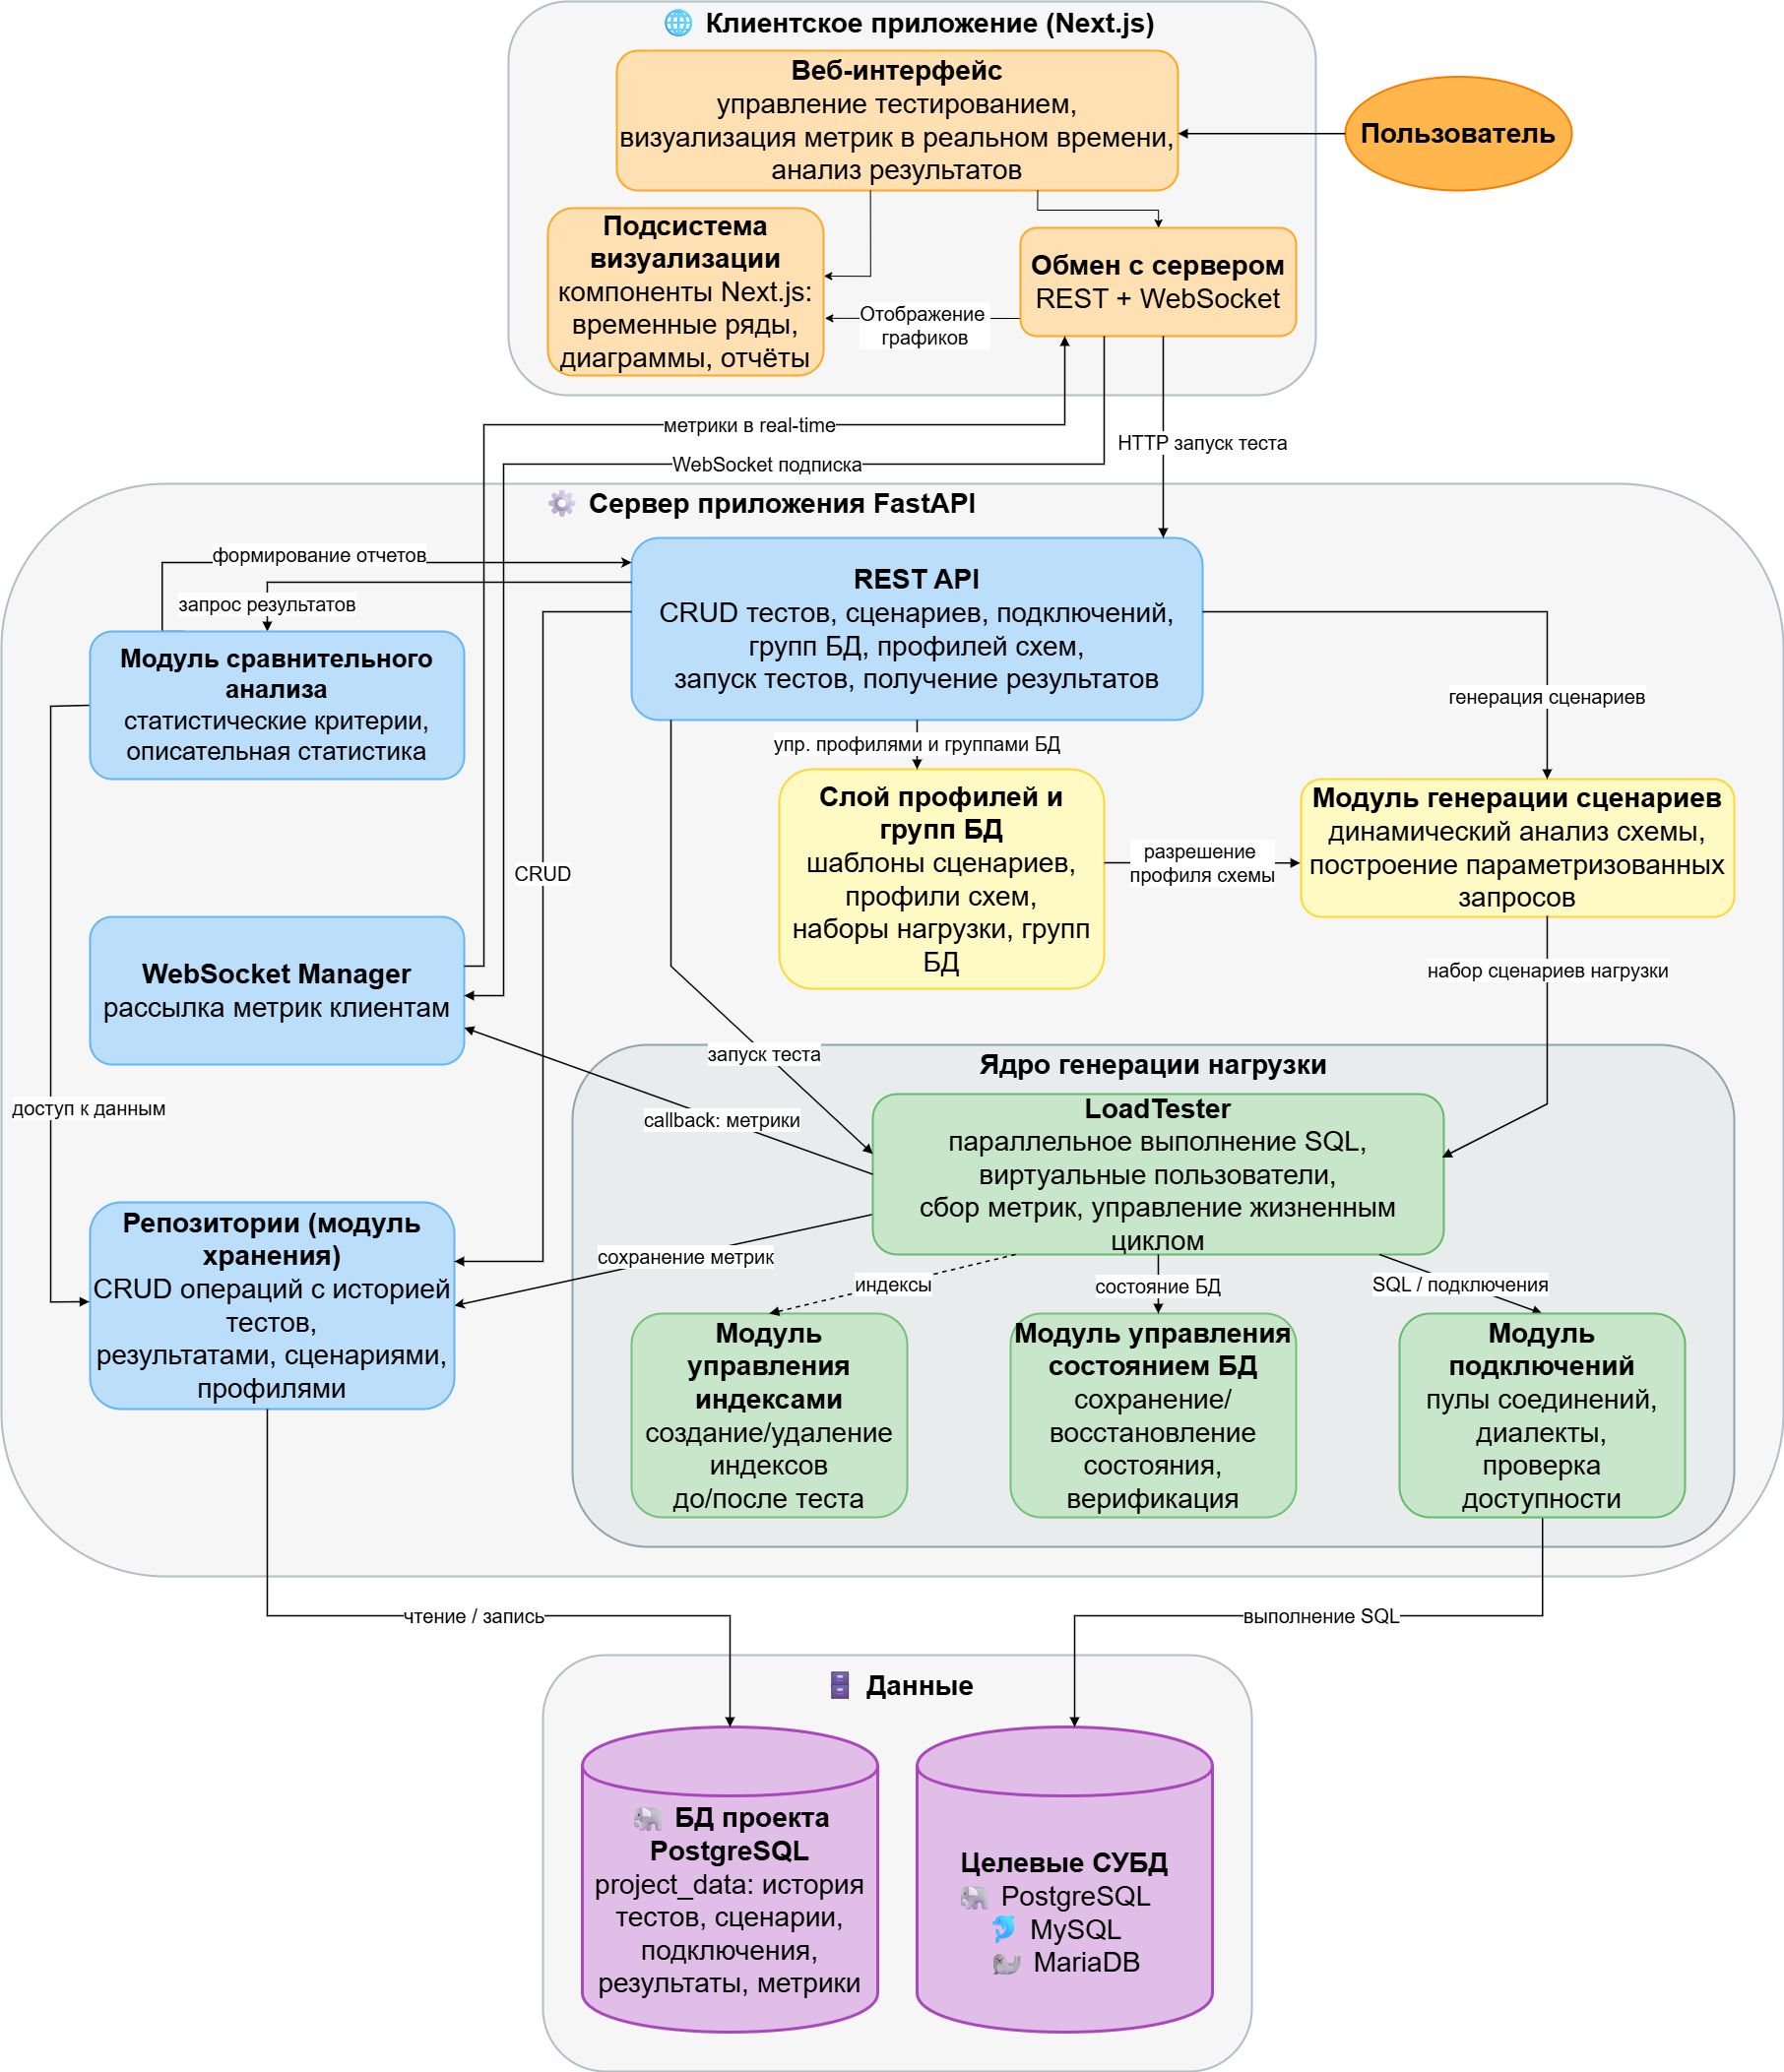
\includegraphics[width=0.9\linewidth]{img/arch.png}
    \caption{Взаимодействие компонентов системы}
    \label{fig:architecture}
\end{figure}

\subsection{Модуль генерации нагрузки и сбора метрик}

Модуль генерации нагрузки является центральным компонентом системы. При его проектировании определялись требования к параллельному выполнению SQL-запросов, точному замеру времени отклика, сбору системных и внутренних метрик СУБД, управлению индексами сценария, а также автоматическому управлению состоянием тестируемых баз данных.

Генерация нагрузки осуществляется с использованием асинхронной модели выполнения на базе библиотеки asyncio. Каждый виртуальный пользователь реализуется как асинхронная задача через \texttt{asyncio.Task}, выполняющая заданное число итераций SQL-запросов. Параллельное выполнение задач обеспечивается функцией \texttt{asyncio.gather()}, которая запускает все задачи одновременно и ожидает их завершения. Такой подход позволяет эффективно использовать ресурсы сервера без создания избыточного числа потоков операционной системы.

Для каждого выполняемого запроса фиксируется время отклика с использованием функции \texttt{time.perf\_counter()}, обеспечивающей высокую точность измерений. Результаты отдельных запросов накапливаются в структуре данных, из которой впоследствии вычисляются агрегированные метрики: среднее время отклика, процентили p50, p95, p99, минимальное и максимальное значения, а также количество ошибок.

Сбор метрик производительности организован в виде отдельного асинхронного цикла, выполняющегося параллельно с генерацией нагрузки. Цикл активируется с интервалом в одну секунду и на каждой итерации выполняет следующие действия:

\begin{enumerate}[label=\arabic*)]
    \item вычисляет агрегированные метрики за прошедший интервал времени на основе накопленных результатов запросов;
    \item собирает системные метрики через библиотеку psutil: загрузку центрального процессора, использование оперативной памяти, интенсивность дискового ввода-вывода, сетевой трафик;
    \item собирает внутренние метрики СУБД: коэффициент попаданий в кэш, количество ожиданий блокировок, количество взаимных блокировок, размеры таблиц;
    \item передаёт собранные метрики через callback-механизм для трансляции в реальном времени и сохранения в базе данных истории.
\end{enumerate}

Для трансляции метрик в реальном времени применяется callback-паттерн, обеспечивающий развязку между модулем генерации нагрузки и подсистемой передачи данных. Метрики сохраняются в базе данных истории в двух форматах: как точки временного ряда для построения графиков и как сырые выборки для последующего статистического анализа. Разделение форматов хранения позволяет применять к одним и тем же данным как визуализацию временны\'х рядов, так и непараметрические статистические критерии.

\subsubsection{Модуль управления индексами}

До начала основного этапа тестирования \texttt{IndexManager} создаёт индексы базы данных в соответствии со спецификацией выбранной конфигурации сценария нагрузки. Каждый индекс описывается объектом \texttt{ScenarioBundleIndex}, содержащим имя таблицы, перечень столбцов, тип индекса, признак уникальности и необязательное условие. После завершения тестового прогона \texttt{IndexManager} удаляет созданные индексы, восстанавливая исходное состояние схемы. Результат каждой операции фиксируется в объекте \texttt{IndexOperationResult}, содержащем информацию о времени создания и удаления каждого индекса, а также список ошибок.

\subsubsection{Алгоритм сохранения и восстановления состояния базы данных}

Тесты с операциями записи изменяют данные в тестируемой базе данных, что исключает повторяемость прогонов без предварительного сброса состояния. Для решения этой проблемы спроектирован модуль управления состоянием базы данных. Перед тестом анализируются SQL-запросы сценария: при наличии write-операций фиксируется снимок состояния базы данных, а после завершения теста данные восстанавливаются до исходного состояния. Для предотвращения конфликтов при параллельном тестировании нескольких баз данных одного типа предусмотрена блокировка на уровне типа СУБД, гарантирующая последовательное выполнение операций сохранения и восстановления.

В системе предусмотрены две взаимозаменяемые стратегии управления состоянием, выбор между которыми задаётся конфигурацией. Нативная стратегия использует штатные CLI-утилиты конкретной СУБД для создания дампа и его последующего восстановления --- этот подход обеспечивает максимальную точность и скорость операций. SQL-стратегия создаёт внутрибазовые копии таблиц средствами самой СУБД и не требует наличия внешних утилит, однако временно увеличивает объём данных в тестируемой базе. Если CLI-утилиты недоступны, система автоматически переключается с нативной стратегии на SQL-стратегию. После восстановления модуль верификации сравнивает число строк и контрольные суммы таблиц с зафиксированным до теста снимком и формирует отчёт о расхождениях при их обнаружении.

\subsubsection{Механизм параметризации запросов}

Для моделирования реалистичной нагрузки реализован механизм параметризации SQL-запросов. Каждый параметр запроса в конфигурации сценария нагрузки может быть сгенерирован одним из следующих способов:

\begin{enumerate}[label=\arabic*)]
    \item \texttt{random\_int} --- случайное целое число из заданного диапазона [min, max];
    \item \texttt{random\_from\_table} --- случайное значение из указанного столбца существующей таблицы базы данных;
    \item \texttt{sequential\_int} --- последовательное целое число, инкрементируемое на каждой итерации;
    \item \texttt{uuid} --- случайно сгенерированный UUID версии 4;
    \item \texttt{fixed} --- фиксированное значение, заданное в конфигурации параметра;
    \item \texttt{random\_string} --- случайная строка заданной длины из алфавитно-цифровых символов;
    \item \texttt{random\_date} --- случайная дата из заданного диапазона.
\end{enumerate}

Такой подход позволяет варьировать данные в запросах и избегать эффектов кэширования планов выполнения, которые могут искажать результаты тестирования. Значения типа \texttt{random\_from\_table} кэшируются на уровне ключа \texttt{db\_key:table:column} для снижения числа дополнительных запросов к БД в ходе теста.

Перед основным этапом тестирования выполняется фаза прогрева warmup, в ходе которой система выполняет серию предварительных запросов для инициализации кэшей и буферов СУБД. Это позволяет исключить влияние начальной инициализации на результаты основного этапа и получить более стабильные и воспроизводимые метрики производительности.

\subsection{Проектирование слоя сценариев и логических баз данных}

Для обеспечения гибкого сопоставления нагрузочных сценариев с конкретными базами данных в системе спроектирован трёхуровневый слой управления сценариями. Данная архитектура позволяет описать логику нагрузки независимо от конкретной СУБД и автоматически подбирать конкретные SQL-запросы при выборе подключения.

Нижний уровень образует шаблон сценария~--- логическое описание вида нагрузки без привязки к конкретной схеме данных. Шаблоны определяют семантику нагрузки: поддерживаются шесть встроенных типов~--- только чтение, только запись, смешанная лёгкая нагрузка, смешанная тяжёлая нагрузка, OLTP и OLAP. Встроенные шаблоны создаются автоматически при инициализации системы.

Средний уровень образует профиль схемы~--- описание структуры данных, общей для группы совместимых баз данных. Профиль связывает набор подключений с конкретной моделью данных и поддерживает три режима привязки: подтверждённый пользователем, ожидающий подтверждения и не определённый. При подключении новой базы данных система автоматически анализирует её схему и предлагает наиболее подходящий профиль с указанием степени уверенности определения.

Верхний уровень образует конфигурация сценария нагрузки~--- конкретная связка профиля схемы и шаблона сценария. Конфигурация содержит перечень параметризованных SQL-запросов и спецификацию индексов. Уникальность пары <<профиль + шаблон>> обеспечивается на уровне модели данных, что гарантирует отсутствие дублирующих активных конфигураций.

Конфигурации сценариев нагрузки формируются динамически на основе реальной схемы подключённой базы данных: система извлекает метаданные таблиц, столбцов и ключей и строит параметризованные SQL-шаблоны для каждого из шести типов нагрузки. При запуске теста конфигурация фиксируется в неизменяемом снимке, который сохраняется вместе с прогоном, обеспечивая воспроизводимость результатов.

Логическая база данных объединяет набор физических подключений под единой логической моделью данных и связывает их с конкретным профилем схемы. Это позволяет тестировать несколько экземпляров одной и той же схемы~--- например, PostgreSQL, MySQL и MariaDB с одинаковой структурой данных~--- в рамках одного прогона без дополнительной настройки сценариев. Система отслеживает совместимость схем подключённых баз данных и формирует отчёт о расхождениях при их обнаружении.

Спроектированный трёхуровневый слой обеспечивает масштабируемость системы: добавление новой схемы данных сводится к созданию профиля и генерации конфигураций сценариев нагрузки без изменения логики генерации нагрузки. Спроектированная архитектура формирует основу для перехода к следующему компоненту системы~--- подсистеме визуализации и сравнительного анализа.

\subsection{Подсистема визуализации и сравнительного анализа}

Подсистема визуализации предназначена для представления результатов нагрузочного тестирования в наглядном виде и обеспечения возможности сравнительного анализа нескольких тестовых прогонов.

Модуль сравнительного анализа поддерживает два режима работы. Режим per\_test предназначен для анализа одного тестового прогона с несколькими подключениями: выполняется попарное сравнение СУБД по метрикам задержки и пропускной способности с ранжированием подключений. Режим series ориентирован на анализ серии прогонов с различными уровнями нагрузки: строятся траектории изменения метрик по уровням и оцениваются характеристики масштабируемости.

В основе сравнительного анализа лежат непараметрические статистические критерии, применение которых обосновано характером распределения задержек: эмпирические распределения времени отклика, как правило, не являются нормальными и содержат выбросы. Тип критерия выбирается автоматически по результатам проверки нормальности выборки. При попарном сравнении нескольких СУБД применяется поправка на множественные сравнения для контроля уровня ложных открытий.

Аналитический отчёт формируется по структурированным правилам и включает краткое резюме с высокоуровневым вердиктом, анализ влияния параметров конфигурации на ключевые метрики, секцию практической значимости различий и конкретные рекомендации. Дополнительно автоматически выявляются характерные паттерны нестабильности производительности, деградации при масштабировании и высоких хвостовых задержек.

Для визуализации результатов сравнения предусмотрены три типа диаграмм: столбчатая диаграмма абсолютных значений задержки (среднее, p95, p99), диаграмма размаха для оценки разброса и асимметрии распределений, а также временно\'й график пропускной способности для выявления нестабильности и трендов. Детали программной реализации модуля сравнительного анализа рассмотрены в разделе~\ref{subsec:comparison_impl}.

\subsection{Модель данных}

Хранение данных системы организовано в базе данных PostgreSQL и включает следующие основные сущности.

TestRun --- запись о тестовом прогоне. Содержит уникальный идентификатор UUID, наименование, статус, конфигурацию теста в формате JSON (типы СУБД, число виртуальных пользователей, число итераций, время прогрева, идентификатор сценария), итоговую статистику в формате JSON, а также ссылку на логическую базу данных и поля управления состоянием базы данных: признак наличия операций записи, перечень затронутых таблиц, статус восстановления, длительность восстановления, ошибки восстановления, результат верификации. Связана с записями TestResult, TimeSeries и MetricSample через внешние ключи с каскадным удалением.

TestResult --- результаты тестирования для одной СУБД в рамках прогона. Содержит идентификатор тестового прогона, тип СУБД, идентификатор запроса, агрегированные метрики производительности в формате JSON (среднее время отклика, p50, p95, p99, TPS, количество ошибок, частота ошибок), системные метрики и внутренние метрики СУБД.

TimeSeries --- точки временного ряда для построения графиков. Каждая запись соответствует одному секундному интервалу тестирования и содержит: идентификатор тестового прогона, тип СУБД, временную метку, значения метрик (время отклика, TPS, загрузка CPU, использование RAM, дисковые IOPS, сетевой трафик, активные соединения, счётчик ошибок).

MetricSample --- сырые выборки метрик для статистического анализа. Каждая запись содержит: идентификатор тестового прогона, тип СУБД, ключ подключения, идентификатор запроса, тип выборки (request\_latency, throughput\_window), временную метку, задержку в миллисекундах, пропускную способность и признак ошибки.

DatabaseConnectionConfig --- конфигурация подключения к СУБД. Содержит тип СУБД, адрес сервера, порт, наименование базы данных, имя пользователя, зашифрованный пароль, группу подключений, идентификатор логической базы данных, идентификатор профиля схемы, а также результаты автоопределения профиля: имя определённого профиля, коэффициент уверенности и источник привязки.

SchemaProfile --- профиль схемы данных, описывающий структуру, общую для группы совместимых баз данных. Содержит наименование, описание, режим определения, ссылку на эталонное подключение, признак встроенного профиля. Связан с подключениями, логическими базами данных и конфигурациями сценариев нагрузки.

LogicalDatabase --- логическая база данных, объединяющая несколько физических подключений под единой моделью данных. Содержит наименование, описание, ссылку на профиль схемы, ссылку на эталонное подключение, статус привязки профиля, статус совместимости подключённых баз данных и отчёт совместимости. Связана с набором \texttt{DatabaseConnectionConfig} и с тестовыми прогонами через поле \texttt{logical\_database\_id} в \texttt{TestRun}.

ScenarioTemplate --- логический шаблон сценария нагрузки. Содержит строковый идентификатор, наименование, описание и признак встроенности. Связан с конфигурациями сценариев нагрузки через отношение <<один ко многим>>.

ScenarioBundle --- конкретная конфигурация сценария нагрузки, объединяющая профиль схемы и шаблон сценария. Содержит наименование, описание, источник генерации, признаки встроенности и активности. Уникальность активной пары <<профиль + шаблон>> обеспечивается частичным уникальным индексом. Связан с перечнями SQL-запросов и индексов.

ScenarioBundleQuery --- SQL-запрос внутри конфигурации сценария нагрузки. Содержит шаблон SQL-запроса, тип запроса, вес и порядковый номер выполнения. Связан с параметрами через отношение <<один ко многим>>.

ScenarioBundleParam --- параметр SQL-запроса внутри конфигурации сценария нагрузки. Содержит наименование параметра, тип генерации значений, диапазоны значений, ссылки на таблицу и столбец базы данных, текущее значение и шаг инкремента.

ScenarioBundleIndex --- спецификация индекса, связанного с конфигурацией сценария нагрузки. Содержит имя таблицы, перечень столбцов, тип индекса, наименование индекса, признак уникальности, условие (для частичных индексов) и описание. Используется \texttt{IndexManager} для создания и удаления индексов при выполнении тестового прогона.

Все основные сущности используют UUID в качестве первичных ключей для обеспечения глобальной уникальности идентификаторов и совместимости в распределённых сценариях. Высоконагруженные таблицы \texttt{TimeSeries} и \texttt{MetricSample} используют \texttt{BigInteger} для первичного ключа с автоинкрементом, что обеспечивает максимальную производительность вставки при потоковой записи метрик.

Модель данных представлена на ER-диаграмме на рисунке~\ref{fig:er_diagram}.

\begin{figure}
    \centering
    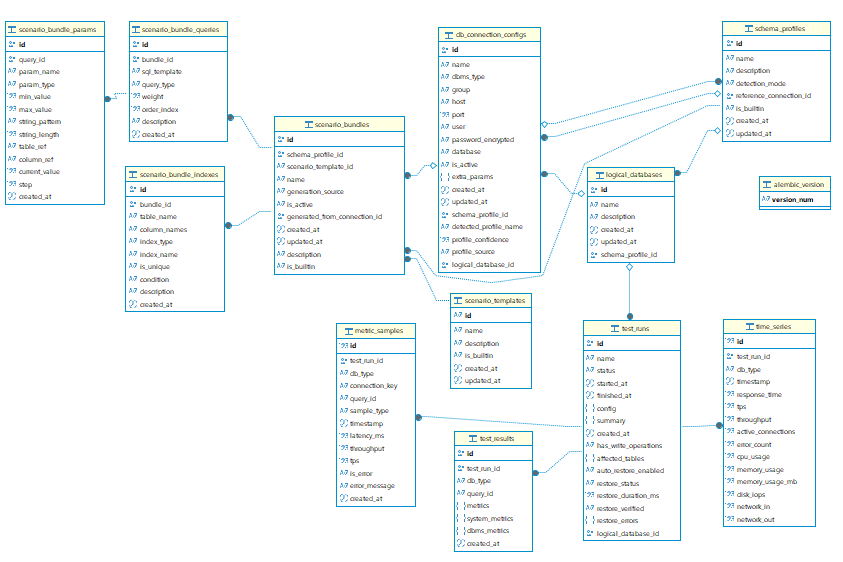
\includegraphics[width=0.9\linewidth]{img/er.png}
    \caption{ER-диаграмма модели данных системы}
    \label{fig:er_diagram}
\end{figure}

Проектирование модели данных с разделением на слой тестовых результатов и слой сценариев/профилей обеспечивает независимую развитие каждой части системы.

Спроектированная архитектура и модель данных создают необходимую основу для программной реализации системы, рассматриваемой в следующей главе. % Глава 2. Проектирование системы
    \section{ПРОГРАММНАЯ РЕАЛИЗАЦИЯ}

\subsection{Выбор и обоснование технологического стека}

На основе спроектированной в предыдущей главе архитектуры была выполнена программная реализация системы. Выбор технологического стека определялся требованиями к производительности, поддерживаемости и удобству разработки. Для серверной части был выбран язык Python версии~3.11 в сочетании с фреймворком FastAPI~\cite{fastapi_docs}. Python обеспечивает высокую скорость разработки благодаря развитой экосистеме библиотек для работы с базами данных, статистического анализа и визуализации. FastAPI предоставляет современный асинхронный веб-фреймворк с автоматической генерацией документации API через OpenAPI, встроенной валидацией данных через Pydantic версии~2 и высокой производительностью, сопоставимой с фреймворками на Node.js. Управление конфигурацией осуществляется через библиотеку pydantic-settings, загружающую параметры из переменных окружения и файла \texttt{.env}.

Для асинхронного выполнения запросов к СУБД выбраны драйверы asyncpg для PostgreSQL и aiomysql для MySQL и MariaDB. Оба драйвера обеспечивают неблокирующий ввод-вывод, что позволяет эффективно обрабатывать множество параллельных соединений в рамках одного потока операционной системы. В качестве ORM-слоя используется SQLAlchemy версии 2.0 с поддержкой асинхронных сессий, что обеспечивает типобезопасную работу с базой данных истории. Для управления миграциями схемы базы данных применяется инструмент Alembic, позволяющий описывать изменения схемы в виде версионируемых Python-скриптов и применять их автоматически при старте приложения.

Для клиентской части выбран фреймворк Next.js версии~16 на базе React~19 с использованием TypeScript. Next.js обеспечивает клиентскую маршрутизацию через App Router и встроенную поддержку серверных компонентов. TypeScript гарантирует типобезопасность на всех уровнях клиентского приложения, снижая количество ошибок времени выполнения. Для управления состоянием приложения выбрана библиотека Zustand, отличающаяся минимальным объёмом кода и отсутствием необходимости в оборачивании приложения в провайдеры. Для визуализации данных используются библиотеки Recharts и Plotly: Recharts предоставляет декларативный API для построения интерактивных графиков на базе SVG, Plotly применяется для диаграмм размаха и расширенных статистических визуализаций. Стилизация реализована через Tailwind CSS версии~4 с CSS-переменными как дизайн-токенами; компоненты интерфейса построены на базе shadcn/ui поверх Radix UI, что обеспечивает доступность и корректную работу с клавиатурой.

Для развёртывания всех компонентов системы используется Docker Compose; состав сервисов, порты и особенности сборки образов рассматриваются в разделе о контейнеризации настоящей главы.

\subsection{Реализация серверной части}

Серверная часть системы реализована в виде модульного приложения FastAPI. Точка входа находится в файле \texttt{main.py}, где инициализируется экземпляр приложения, регистрируются маршруты и создаётся WebSocket-эндпоинт.

Инициализация компонентов системы выполняется через модуль \texttt{initialize.py}, который создаёт экземпляры пяти репозиториев: \texttt{TestRepository}, \texttt{ConnectionRepository}, \texttt{ProfileRepository}, \texttt{ScenarioBundleRepository} и \texttt{DatabaseGroupRepository}. Каждый репозиторий принимает URL базы данных истории и создаёт собственный пул асинхронных соединений через SQLAlchemy. Настройки стратегии восстановления баз данных \texttt{settings.restore.*} загружаются из модуля конфигурации \texttt{core/config.py} и изменяются через \texttt{settings\_routes} без отдельного репозитория. Такой подход реализует паттерн внедрения зависимостей и обеспечивает централизованное управление жизненным циклом компонентов. При недоступности базы данных инициализация не прерывает запуск приложения~--- репозитории устанавливаются в \texttt{None}, а соответствующая функциональность корректно деградирует.

Запуск и остановка приложения управляются через менеджер контекста lifespan. При запуске выполняются два последовательных шага:

\begin{enumerate}[label=\arabic*)]
    \item автоматически применяются миграции Alembic командой \texttt{upgrade head}, что гарантирует актуальность схемы базы данных вне зависимости от версии развёртывания;
    \item при успешной инициализации всех трёх ключевых репозиториев: \texttt{connection\_repository}, \texttt{profile\_repository} и \texttt{scenario\_bundle\_repository}~--- запускается \texttt{LogicalScenarioBootstrap}: он создаёт шесть встроенных шаблонов сценариев и профили схем, а при наличии зарегистрированных подключений с определёнными профилями~--- генерирует SQL-наборы для пяти шаблонов с автогенерацией и встроенные OLTP-наборы для поддерживаемых профилей.
\end{enumerate}

Первый шаг является fail-fast: при возникновении ошибки Alembic запуск приложения немедленно прерывается, что исключает работу системы с устаревшей схемой базы данных. Bootstrap на втором шаге выполняется условно~--- только при наличии рабочего подключения к базе данных проекта; если база данных недоступна, bootstrap пропускается без прерывания запуска. Повторный запуск обоих шагов не создаёт дублирующих записей~--- процедура полностью идемпотентна.

\subsubsection{Модуль генерации нагрузки}

Модуль генерации нагрузки реализован в классе \texttt{LoadTester} файла \texttt{load\_tester/tester.py}. Основным методом запуска является \texttt{run\_resolved\_scenario\_test\_suite}, принимающий разрешённый набор сценария нагрузки и список идентификаторов подключений. В зависимости от типа набора метод выполняет либо одиночные SQL-запросы, либо транзакционные последовательности операций, где каждый виртуальный пользователь атомарно выполняет группу инструкций изменения данных. Единая структура каждого прогона: подготовка базы данных, двухфазный прогрев, измерительная фаза, сбор метрик, восстановление состояния, верификация. Блок \texttt{try/finally} гарантирует выполнение восстановления даже при возникновении ошибок в ходе тестирования.

Базовый метод \texttt{execute\_query} выполняет отдельный SQL-запрос к указанной базе данных, замеряя время отклика через \texttt{time.perf\_counter()}. На рисунке~\ref{lst:execute_query} приведён фрагмент реализации:

\begin{figure}
    \begin{minipage}{\linewidth}
\begin{lstlisting}
async def execute_query(self, db_key, query, query_id):
    """ Выполнение одного запроса с измерением времени """
    start_time = time.perf_counter()
    error = None
    rows_count = 0
    db_type = self.db_connection.get_dbms_type(db_key)

    try:
        engine = await self.db_connection.get_engine_async(db_key)
        async with engine.connect() as conn:
            result = await conn.execute(text(query))
            rows_count = len(result.fetchall()) if result.returns_rows else 0
            await conn.commit()
    except Exception as e:
        error = str(e)

    end_time = time.perf_counter()
    execution_time = (end_time - start_time) * 1000

    return {
        'query_id': query_id,
        'execution_time_ms': execution_time,
        'rows_count': rows_count,
        'error': error,
        'timestamp': datetime.now(timezone.utc).isoformat()
    }
\end{lstlisting}
    \end{minipage}
    \caption{Реализация метода \texttt{execute\_query} класса LoadTester}
    \label{lst:execute_query}
\end{figure}

Использование \texttt{time.perf\_counter()} обеспечивает высокую точность замеров; асинхронное подключение через SQLAlchemy engine позволяет выполнять запросы без блокировки потока; результат включает не только время выполнения, но и количество обработанных строк и текст ошибки при её возникновении.

Каждый виртуальный пользователь реализован как асинхронная задача \texttt{asyncio.Task}. На каждой итерации выполняется одиночный запрос или транзакционная последовательность операций в соответствии с \texttt{workload\_mode} разрешённого набора сценария; результаты накапливаются в буфере. При достижении интервала в одну секунду вычисляются агрегированные метрики окна: среднее время отклика, успешная и полная пропускная способность, количество успешных и ошибочных операций; итог прогона дополняется перцентилями p50, p95, p99, минимумом, максимумом и стандартным отклонением за измерительную фазу. Данные передаются через callback-механизм для трансляции в WebSocket и сохранения в базу данных истории.

Для сбора системных метрик используется метод \texttt{get\_system\_metrics}, который через библиотеку \texttt{psutil} получает загрузку центрального процессора (проценты), использование оперативной памяти (проценты и мегабайты), дисковые операции в секунду, скорости чтения и записи (МиБ/с), а также входящий и исходящий сетевой трафик (МиБ/с). Метод \texttt{get\_dbms\_metrics} через слой диалектов в каталоге \texttt{database/dialects/} возвращает унифицированный набор внутренних показателей: коэффициент попаданий в кэш, размер буферного пула (мегабайты и метка параметра), число ожиданий блокировок и взаимных блокировок, объёмы таблиц. Для PostgreSQL используются представления \texttt{pg\_stat\_database}~\cite{postgresql_docs} и \texttt{pg\_stat\_bgwriter}, для MySQL и MariaDB~--- \texttt{performance\_schema.data\_lock\_waits} и \texttt{SHOW GLOBAL STATUS}. Слой диалектов изолирует СУБД-специфичную логику и позволяет расширять поддержку СУБД без изменения основного цикла сбора метрик.

\subsubsection{Модуль генерации сценариев}

Модуль генерации сценариев реализован в классе \texttt{ScenarioGenerator} файла \texttt{database/scenario\_generator.py}. Генератор принимает на вход подключение к целевой СУБД и тип шаблона сценария, анализирует метаданные схемы через \texttt{SchemaAnalyzer} и формирует структуру \texttt{ScenarioBundle} с массивами запросов и индексов.

Для пяти встроенных шаблонов с автогенерацией, кроме OLTP, \texttt{ScenarioGenerator} строит параметризованные SQL-шаблоны: шаблон только чтения включает выборки по первичному ключу и JOIN-запросы по внешним ключам, только записи~--- операции INSERT и UPDATE на изменяемых таблицах, смешанные шаблоны~--- комбинации SELECT и UPDATE с различными весами, аналитические запросы~--- агрегации, JOIN и диапазонные чтения по метаданным схемы. Шаблон OLTP не проходит через генератор: для профилей Sakila и Brazilian E-Commerce наборы транзакций задаются встроенными конфигурациями. Параметры запросов типа \texttt{random\_from\_table} ссылаются на реальные столбцы схемы и кэшируются по ключу \texttt{db\_key:table:column}. Класс \texttt{ScenarioBundleResolver} разрешает конкретный набор сценария нагрузки при запуске теста: по идентификатору набора или по паре <<профиль + шаблон>> он загружает запросы, параметры и индексы, формируя неизменяемый снимок конфигурации, который сохраняется вместе с прогоном для воспроизводимости.

\subsubsection{Callback-механизм потоковой передачи данных}

Ниже детализирован callback-механизм потоковой передачи метрик, упомянутый при описании \texttt{LoadTester}. Для связи с WebSocket и базой данных истории используется паттерн Observer. Класс \texttt{LoadTester} поддерживает два независимых callback: callback метрик, вызываемый на каждой итерации сбора агрегированных показателей, и callback статуса операций сохранения/восстановления состояния базы данных. Такое разделение позволяет клиенту независимо отслеживать ход теста и состояние данных.

Класс \texttt{TestStreamingCallback} файла \texttt{websocket\_manager.py} выступает в роли наблюдателя: он получает метрики от \texttt{LoadTester} и транслирует их подписчикам. Метод формирует объект \texttt{TestMetricsUpdate}, содержащий все метрики производительности, системные показатели и прогресс выполнения. Данные передаются через \texttt{ConnectionManager} для рассылки всем WebSocket-подписчикам теста и одновременно сохраняются в базе данных истории как точка временного ряда. Для оптимизации записи сырых выборок метрик используется буферизация: накопление происходит до достижения размера буфера в 10 записей, после чего выполняется пакетная вставка через метод \texttt{add\_metric\_sample\_batch}.

\subsubsection{Управление WebSocket-соединениями}

Управление WebSocket-соединениями реализовано в классе \texttt{ConnectionManager} файла \texttt{websocket\_manager.py}. Класс хранит активные соединения в словаре \texttt{active\_connections}, ключом которого является идентификатор теста, а значением~--- список WebSocket-объектов. Метод \texttt{connect} принимает новое соединение и добавляет его в список, метод \texttt{disconnect} удаляет соединение и очищает пустые списки. Метод \texttt{broadcast\_to\_test} рассылает JSON-сообщение всем подписчикам конкретного теста. WebSocket-эндпоинт зарегистрирован по пути \texttt{/ws/test/\{test\_id\}} и обрабатывает входящие ping-сообщения от клиента для поддержания соединения.

\subsubsection{Управление состоянием базы данных}

Оркестратор управления состоянием баз данных реализован в классе \texttt{DatabaseStateManager} файла \texttt{database/state\_manager.py}. Класс управляет полным жизненным циклом операций: анализ запросов сценария, сохранение состояния базы данных, выполнение теста, восстановление исходных данных и верификация целостности.

Метод \texttt{prepare\_for\_test} сначала передаёт SQL-запросы сценария в модуль \texttt{QueryAnalyzer}, который определяет наличие write-операций INSERT, UPDATE и DELETE. Если сценарий содержит только SELECT-запросы, подготовка пропускается. При обнаружении write-операций определяются затронутые таблицы и полный список всех таблиц базы данных. Затем модуль \texttt{StateVerifier} фиксирует объект \texttt{StateFingerprint}~--- количество строк в каждой таблице, значения последовательностей и, при включённой настройке \texttt{verify\_checksums}, контрольные суммы данных,~--- который впоследствии используется для верификации восстановления. После этого через настроенную стратегию сохраняется состояние всех таблиц базы данных: не только затронутых write-операциями, но и всех остальных, что гарантирует полный откат к исходному состоянию.

Нативная стратегия \texttt{NativeDumpStrategy} является основной: она вызывает CLI-утилиты конкретной СУБД~--- \texttt{pg\_dump} для создания дампа и \texttt{pg\_restore}/\texttt{psql} для восстановления у PostgreSQL; \texttt{mysqldump}/\texttt{mysql} для MySQL; \texttt{mariadb-dump}/\texttt{mariadb} для MariaDB,~--- сохраняя результат в виде файла дампа в директории \texttt{snapshots}. Для MariaDB используется самостоятельный клиент \texttt{mariadb-dump} с приоритетом перед \texttt{mysqldump}: это обеспечивает корректную обработку DEFINER-клауз и специфических расширений синтаксиса. При восстановлении через нативную стратегию для MySQL/MariaDB дамп предварительно очищается от DEFINER-клауз, а для PostgreSQL выполняется TRUNCATE целевых таблиц перед data-only восстановлением через \texttt{pg\_restore}/\texttt{psql}. Если CLI-утилиты не обнаружены в PATH, \texttt{NativeDumpStrategy} автоматически переключается на \texttt{SqlBackupStrategy}.

SQL-стратегия \texttt{SqlBackupStrategy} создаёт внутрибазовые копии таблиц через запросы вида \texttt{CREATE~TABLE~\ldots~AS~SELECT~*} с фиксированным префиксом \texttt{\_loadtest\_backup\_} в той же схеме. При восстановлении таблицы очищаются через TRUNCATE и заполняются данными из копий через INSERT; порядок восстановления определяется топологической сортировкой по FK-зависимостям с временным отключением FK-ограничений. Данная стратегия не требует внешних утилит и работает через SQLAlchemy с любой поддерживаемой СУБД, однако временно увеличивает объём данных в тестируемой базе.

Метод \texttt{restore\_after\_test} выполняет восстановление под блокировкой \texttt{asyncio.Lock}, специфичной для типа СУБД, что исключает конфликты при параллельном тестировании. При включённой настройке \texttt{verify\_after\_restore} модуль \texttt{StateVerifier} строит новый \texttt{StateFingerprint} и сравнивает его с исходным: при полном совпадении числа строк и контрольных сумм восстановление считается успешным, при несовпадении формируется отчёт о расхождениях. По завершении операции внутрибазовые копии или временные файлы дампов удаляются.

\subsubsection{Разрешение наборов сценариев нагрузки и запуск теста}

Фоновая задача \texttt{run\_test\_with\_streaming} создаёт экземпляр \texttt{LoadTester}, устанавливает callback для потоковой передачи метрик и callback статуса операций сохранения/восстановления состояния, разрешает набор сценария нагрузки через \texttt{ScenarioBundleResolver} и передаёт его в \texttt{LoadTester} вместе со списком идентификаторов подключений. Перед началом теста \texttt{IndexManager} создаёт индексы, описанные в \texttt{ScenarioBundleIndex}; по завершении теста индексы удаляются. По завершении результаты собираются, сохраняются в базе данных, а статус обновляется на \texttt{completed} или \texttt{failed}. При передаче параметра \texttt{database\_group\_id} тестовый прогон автоматически привязывается к соответствующей группе баз данных.

\subsubsection{Модуль сравнительного анализа}

Модуль сравнительного анализа реализован в классе \texttt{ComparisonService} файла \texttt{comparison/service.py}. Конструктор класса принимает три репозитория: \texttt{repository} для загрузки данных тестов, \texttt{scenario\_bundle\_repository} для получения информации о наборах сценариев нагрузки и \texttt{connection\_repository} для получения данных о подключениях. Основной метод \texttt{analyze} принимает объект \texttt{ComparisonRequest} с полями \texttt{analysis\_mode}, \texttt{test\_ids}, необязательным \texttt{baseline\_id} и конфигурацией отчёта.

При обнаружении потенциальных проблем сопоставимости~--- разных наборов сценариев нагрузки, неравных временных периодов, смешанных типов СУБД~--- система формирует предупреждения, включаемые в итоговый отчёт.

Метод \texttt{analyze} маршрутизирует запрос по полю \texttt{analysis\_mode}, задаваемому клиентом на странице истории тестов. В режиме \texttt{per\_test} передаётся ровно один идентификатор прогона: загружаются его конфигурация, результаты и сырые выборки метрик по каждому подключению с ключом \texttt{connection\_key}; для всех пар СУБД внутри прогона вычисляется описательная статистика задержки и пропускной способности, применяются статистические критерии с FDR-поправкой и формируется ранжирование; отчёт генерирует \texttt{PerTestReportGenerator}. В режиме \texttt{series} передаётся от двух до пяти идентификаторов прогонов с различными уровнями нагрузки: для каждой СУБД строятся траектории метрик, оцениваются показатели масштабируемости \texttt{stability\_index}, \texttt{elasticity} и точка насыщения, тренды проверяются критериями Спирмена и Манна--Кендалла; базовый прогон задаётся полем \texttt{baseline\_id}; отчёт генерирует \texttt{SeriesReportGenerator}. Оба генератора реализованы в модуле \texttt{analysis/report\_generator.py}.

Сбор сырых выборок метрик реализован с трёхуровневым механизмом fallback: при наличии записей \texttt{MetricSample} используются они; при их отсутствии~--- данные из \texttt{TimeSeries}; в крайнем случае~--- агрегированные метрики из \texttt{TestResult} с соответствующим предупреждением о сниженной надёжности анализа. Это обеспечивает работоспособность сравнения даже для тестов, выполненных до добавления модуля сбора сырых метрик.

Отчёт в режиме \texttt{per\_test} включает краткое резюме с лидером по пропускной способности и СУБД с наименьшей средней задержкой, попарные сравнения с интерпретацией и ранжирование подключений. Отчёт в режиме \texttt{series} дополняется блоком \texttt{parameter\_impacts} с анализом влияния различий конфигурации между прогонами; в обоих режимах автоматически выявляются паттерны нестабильности при высоком CV, деградации при масштабировании и высоких хвостовых задержек при соотношении p99 к медиане.

\subsubsection{Реализация статистических функций}

Модуль \texttt{comparison/statistics.py} содержит математический аппарат для статистического сравнения выборок. Функция \texttt{calculate\_descriptive\_stats} вычисляет описательную статистику через \texttt{numpy}: количество, среднее, медиану, стандартное отклонение, минимум, максимум, процентили p50, p95, p99, коэффициент вариации CV, а также межквартильный размах IQR. Функция \texttt{check\_normality} проверяет нормальность распределения через критерий Шапиро--Уилка с ограничением выборки в 5000 элементов.

Функция \texttt{compare\_two\_samples} реализует двухэтапный алгоритм выбора критерия. На первом этапе проверяется размер выборки: если количество элементов менее~10, статистический тест не выполняется и выводится предупреждение о недостаточном объёме данных; если размер выборки превышает 5000~элементов, из неё извлекается случайная подвыборка для снижения вычислительной нагрузки. Затем к полученной выборке применяется критерий Шапиро--Уилка: если p-значение превышает 0,05, нулевая гипотеза о нормальности не отвергается. На втором этапе по результату проверки нормальности выбирается критерий сравнения: при нормальном распределении применяется критерий Уэлча, не требующий равенства дисперсий; при ненормальном~--- критерий Манна--Уитни, являющийся непараметрическим аналогом t-критерия. Если p-значение выбранного критерия оказывается меньше~0,05, различие признаётся статистически значимым и формируется текстовая интерпретация с указанием процентного отклонения. При сравнении нескольких пар применяется FDR-поправка Бенджамини--Хохберга для контроля уровня ложных открытий.

\subsubsection{Реализация REST API}

REST API системы разделено на восемь модулей маршрутов, каждый из которых отвечает за свою область функциональности. Основные эндпоинты представлены в таблице~\ref{tab:api_endpoints}.

\begin{table}
    \centering
    \caption{Основные эндпоинты REST API}
    \label{tab:api_endpoints}
    \begin{tabularx}{\textwidth}{|>{\RaggedRight}X|>{\RaggedRight}X|>{\RaggedRight}X|}
        \hline
        Модуль & Метод и путь & Назначение \\
        \hline
        test & POST /test/async & Асинхронный запуск теста \\
        \hline
        test & GET /test/async/\{id\} & Получение статуса теста \\
        \hline
        test & GET /test/async/\{id\}/results & Получение результатов \\
        \hline
        history & GET /history/tests & Список тестов с пагинацией \\
        \hline
        history & GET /history/tests/\{id\} & Детали конкретного теста \\
        \hline
        history & DELETE /history/tests/\{id\} & Удаление теста \\
        \hline
        connection & GET /api/connections & Список подключений \\
        \hline
        connection & POST /api/connections & Создание подключения \\
        \hline
        connection & POST /api/connections/test & Тестирование подключения \\
        \hline
        database\_state & POST /.../\{id\}/backup & Сохранение состояния базы данных \\
        \hline
        database\_state & POST /.../\{id\}/restore & Восстановление состояния базы данных \\
        \hline
        database\_state & GET /.../\{id\}/estimate & Оценка объёма данных базы \\
        \hline
        comparison & POST /api/comparison/analyze & Сравнительный анализ \\
        \hline
        schema-profiles & GET /api/schema-profiles & Список профилей схемы \\
        \hline
    \end{tabularx}
\end{table}

\begin{table}
    \centering
    \ContinuedFloat
    \caption*{Продолжение таблицы \ref{tab:api_endpoints}}
    \label{tab:api_endpoints_continue}
    \begin{tabularx}{\textwidth}{|>{\RaggedRight}X|>{\RaggedRight}X|>{\RaggedRight}X|}
        \hline
        schema-profiles & POST /api/schema-profiles & Создание профиля \\
        \hline
        schema-profiles & GET /.../\{id\}/bundles & наборы сценариев нагрузки профиля \\
        \hline
        schema-profiles & POST /.../\{id\}/bundles/generate & Генерация набора сценария нагрузки для профиля схемы \\
        \hline
        database-groups & GET /api/database-groups & Список групп баз данных \\
        \hline
        database-groups & POST /api/database-groups & Создание группы баз данных \\
        \hline
        database-groups & PUT /.../\{id\}/profile & Привязка профиля схемы к группе \\
        \hline
        database-groups & POST /.../\{id\}/bundles/generate & Генерация набора сценария нагрузки для профиля, привязанного к группе баз данных \\
        \hline
        database-groups & POST /.../\{id\}/connections/\allowbreak\{connection\_id\}/confirm-profile & Подтверждение профиля схемы для подключения в группе \\
        \hline
        database-groups & PUT /.../\{id\}/reference-connection & Обновление эталонного подключения \\
        \hline
        settings & GET /api/settings/restore & Настройки восстановления \\
        \hline
        settings & PUT /api/settings/restore & Обновление настроек восстановления \\
        \hline
    \end{tabularx}
\end{table}

Эндпоинты \texttt{POST /.../\{id\}/bundles/generate} в модулях \texttt{schema-profiles} и \texttt{database-groups} вызывают одну операцию генерации наборов сценариев нагрузки через \texttt{ScenarioGenerator}; различаются контекст запроса и проверки входных параметров.

Эндпоинт \texttt{POST /test/async} принимает параметры нагрузки, создаёт запись прогона со статусом \texttt{pending}, запускает фоновую задачу \texttt{run\_test\_with\_streaming} через \texttt{BackgroundTasks} FastAPI и возвращает клиенту \texttt{test\_id} с \texttt{websocket\_url} для подписки на метрики. Настройки стратегии восстановления по пути \texttt{/api/settings/restore} изменяются в памяти процесса до рестарта бэкенда.

\subsubsection{Обработка ошибок}

Обработка ошибок в серверной части реализована на нескольких уровнях. На уровне API маршрутов все исключения перехватываются и преобразуются в HTTP-статусы: \texttt{ValueError}~--- в 400 Bad Request, неожиданные исключения~--- в 500 Internal Server Error. На уровне бизнес-логики ошибки логируются с указанием контекста и, где возможно, обрабатываются без прерывания выполнения теста. Блок \texttt{try/finally} в методах тестирования гарантирует выполнение восстановления базы данных даже при критических ошибках.

При возникновении ошибки выполнения SQL-запроса метод \texttt{execute\_query} не прерывает цикл итераций, а сохраняет текст ошибки в результате и продолжает выполнение следующих запросов. Это позволяет получить полную картину производительности, включая частоту ошибок, которая сама по себе является важной метрикой.

\subsubsection{Слой доступа к данным}

Слой доступа к данным реализован через паттерн Repository. Базовый класс \texttt{BaseRepository} обеспечивает асинхронное подключение к базе данных истории через SQLAlchemy с управлением сессиями через контекстный менеджер. Наследники реализуют специфичные операции для своих сущностей: \texttt{TestRepository} управляет тестовыми прогонами и временными рядами, \texttt{ConnectionRepository}~--- конфигурациями подключений с расшифровкой паролей, \texttt{ProfileRepository}~--- профилями схем и шаблонами сценариев, \texttt{ScenarioBundleRepository}~--- наборами сценариев нагрузки с их запросами и индексами, \texttt{DatabaseGroupRepository}~--- группами баз данных.

Метод \texttt{TestRepository.add\_metric\_sample\_batch} выполняет пакетное сохранение сырых выборок метрик. Код метода приведён на рисунке~\ref{lst:save_metric_samples}:

\begin{figure}
    \begin{minipage}{\linewidth}
\begin{lstlisting}
async def add_metric_sample_batch(
    self, test_run_id: str, samples: List[Dict]
):
    """ Пакетное сохранение сырых метрик """
    if not samples:
        return

    async with self.get_session() as session:
        records = [
            MetricSample(
                test_run_id=test_run_id,
                db_type=s['db_type'],
                connection_key=s['connection_key'],
                query_id=s.get('query_id'),
                sample_type=s.get('sample_type'),
                timestamp=s['timestamp'],
                latency_ms=s.get('latency_ms'),
                throughput=s.get('throughput'),
                is_error=s.get('is_error', False),
                error_message=s.get('error_message'),
            )
            for s in samples
        ]
        session.add_all(records)
        await session.commit()
\end{lstlisting}
    \end{minipage}
    \caption{Метод addMetricSampleBatch класса TestRepository}
    \label{lst:save_metric_samples}
\end{figure}

Пакетная вставка снижает количество обращений к базе данных при высокой интенсивности тестирования. Каждая запись содержит тип выборки, что позволяет гибко выбирать уровень детализации данных при сравнительном анализе.

\subsubsection{Управление подключениями к СУБД}

Класс \texttt{DatabaseConnection} файла \texttt{database/connection.py} управляет подключениями к тестируемым СУБД. Подключения хранятся в репозитории базы данных истории и загружаются лениво при первом асинхронном вызове.

Метод \texttt{\_resolve\_connection\_key} обеспечивает поддержку shorthand-ключей: если передан ключ \texttt{mysql} или \texttt{postgresql} и существует ровно одно активное подключение данного типа, оно используется автоматически. При наличии нескольких подключений одного типа требуется явное указание \texttt{connection\_id}. Кэширование конфигураций подключений в памяти исключает повторные обращения к базе данных при каждом запросе.

Для шифрования паролей подключений используется модуль \texttt{core/crypto.py}, реализующий симметричное шифрование в формате Fernet. Пароль шифруется перед сохранением в базе данных и расшифровывается при установлении подключения к тестируемой СУБД. Ключ шифрования задаётся через переменную окружения \texttt{ENCRYPTION\_KEY}.

\subsection{Реализация клиентской части}

Клиентская часть системы реализована как одностраничное приложение на базе Next.js~16 с клиентской маршрутизацией. Главная страница в файле \texttt{app/page.tsx} определяет компонент-маршрутизатор, который условно отображает один из восьми компонентов-страниц в зависимости от значения \texttt{currentPage} в Zustand store. Общая компоновка включает верхнюю панель с логотипом и навигацией, боковое меню с переключением страниц и основную область контента.

\subsubsection{Архитектура компонентов}

Страница \texttt{HomePage} является стартовой и предоставляет краткое описание системы с кнопками быстрого перехода к конфигурации теста или истории. \texttt{ConnectionsPage} обеспечивает полный CRUD для сохранённых подключений к СУБД: добавление, редактирование, удаление, проверка доступности. При создании подключения страница отображает результат автоопределения профиля схемы с коэффициентом уверенности.

Страница \texttt{ConfigPage} является центральным узлом конфигурации теста. Она содержит несколько карточек: выбор группы баз данных или отдельных подключений, выбор режима теста, выбор сценария или набор сценария нагрузки, настройка параметров нагрузки: числа виртуальных пользователей, числа итераций и времени прогрева, а также сводка конфигурации и кнопка запуска.

Страница \texttt{ScenariosPage} предоставляет браузер наборов сценариев нагрузки через компонент \texttt{logical-scenarios-browser}. В браузере отображаются группы баз данных, профили схем и связанные с ними наборы сценариев нагрузки с их SQL-запросами, параметрами и спецификацией индексов. Предусмотрены операции создания, редактирования, клонирования и генерации наборов сценариев нагрузки из эталонного подключения. Для каждой группы баз данных отображаются статусы \texttt{profile\_status} и \texttt{compatibility\_status}, что позволяет пользователю контролировать состояние привязки профиля и совместимость подключённых баз данных.

Страница \texttt{DashboardsPage} предоставляет дашборд реального времени с четырьмя вкладками: время отклика и пропускная способность, внутренние метрики СУБД, объёмы данных и системные метрики хоста. Каждая вкладка отображает секундные временны\'е ряды для всех подключений группы одновременно.

Страница \texttt{HistoryPage} отображает таблицу выполненных тестов с возможностью выбора одного теста для режима \texttt{per\_test} или от двух до пяти~--- для режима \texttt{series}. Страница \texttt{ComparisonPage} визуализирует ответ \texttt{POST /api/comparison/analyze}: резюме, таблицу метрик~--- в режиме \texttt{per\_test} отклонения относительно первого подключения в порядке \texttt{connection\_ids} прогона, в режиме \texttt{series}~--- относительно базового прогона,~--- диаграммы, статистические тесты, аналитический отчёт и при \texttt{series} блок \texttt{parameter\_impacts}; экспорт результата в JSON выполняется кнопкой Download на той же странице. Страница \texttt{DatabaseStatePage} предоставляет панель ручного сохранения и восстановления состояния подключённых баз данных и оценки объёма данных.

\subsubsection{Управление состоянием}

Состояние приложения хранится в едином store, реализованном через библиотеку Zustand. Файл \texttt{lib/store.ts} определяет интерфейс \texttt{AppState} и создаёт store через \texttt{create<AppState>}. Store включает следующие группы данных: навигация~--- текущая страница и состояние боковой панели; конфигурация теста~--- режим, сценарий, идентификатор набора сценария нагрузки или шаблона, признак использования индексов, число виртуальных пользователей, итерации и время прогрева; текущий тест; история тестов; данные реального времени~--- временные ряды для каждого подключения; словари имён и типов подключений; параметры сравнительного анализа.

Метод \texttt{addRealtimeData} обеспечивает добавление точек временного ряда с ограничением буфера.

Метод \texttt{.slice(-100)} ограничивает массив последними 100 точками для каждого подключения, что предотвращает чрезмерное потребление памяти при длительных тестах и обеспечивает плавную отрисовку графиков. Ключом в словаре \texttt{realtimeData} выступает уникальный идентификатор подключения, что позволяет отображать метрики для нескольких экземпляров одного типа СУБД независимо.

\subsubsection{Реализация WebSocket-хука}

Хук \texttt{useTestWebSocket} файла \texttt{hooks/use-test-websocket.ts} обеспечивает двустороннюю связь с сервером для получения метрик в реальном времени. При монтировании компонента с валидным \texttt{testId} автоматически устанавливается WebSocket-соединение по адресу \texttt{/ws/test/\{testId\}}. Каждые 30 секунд отправляется ping-сообщение для предотвращения разрыва соединения из-за таймаута.

При разрыве соединения во время выполнения теста производится автоматическое переподключение с интервалом 3 секунды. Переподключение выполняется только при статусе \texttt{running}, что предотвращает бесконечные попытки подключения после завершения теста. При получении сообщения типа \texttt{metrics} данные преобразуются в \texttt{TimeSeriesPoint} и добавляются в store через \texttt{addRealtimeData}, что вызывает реактивное обновление компонентов дашборда.

\subsubsection{Модульный API-клиент}

API-клиент реализован как класс \texttt{ApiClient} файла \texttt{lib/api/client.ts}. Базовый URL определяется переменной окружения \texttt{NEXT\_PUBLIC\_API\_URL}. Метод \texttt{request<T>} централизует обработку ошибок: при получении HTTP-статуса, отличного от 2xx, из ответа извлекается сообщение об ошибке и выбрасывается исключение \texttt{Error}. Все методы клиента типизированы через дженерики TypeScript, что обеспечивает проверку корректности данных на этапе компиляции.

Класс включает доменные методы для каждой группы эндпоинтов: методы управления подключениями и их профилями, методы работы с профилями схемы, методы управления группами баз данных, а также методы запуска тестов, получения истории и запуска сравнительного анализа. Экземпляр \texttt{apiClient} экспортируется как singleton; компоненты импортируют методы через barrel-экспорт \texttt{lib/api.ts}.

\subsubsection{Визуализация данных}

Визуализация метрик реализована с использованием библиотек Recharts и Plotly. Секундные ряды дашборда отображаются в переиспользуемом компоненте \texttt{TimeSeriesChart}; подписи пропускной способности зависят от \texttt{workload\_mode} прогона. На странице сравнительного анализа для диаграмм размаха и расширенных статистических графиков применяется Plotly.

Стилизация интерфейса выполнена через Tailwind CSS v4 с использованием дизайн-токенов для цветов, отступов и размеров шрифтов; поддерживается тёмная тема через \texttt{className="dark"} на корневом элементе. Компоненты интерфейса построены на базе Radix UI через библиотеку shadcn/ui. Уведомления пользователю отображаются через библиотеку Sonner в виде всплывающих сообщений.

\subsection{Контейнеризация и развёртывание}

Развёртывание системы организовано через Docker Compose. Основной файл \texttt{docker-compose.yml} определяет три сервиса и представлен в таблице~\ref{tab:docker_services}.

\begin{table}
    \centering
    \caption{Сервисы Docker Compose}
    \label{tab:docker_services}
    \begin{tabularx}{\textwidth}{|>{\RaggedRight}X|>{\RaggedRight}X|>{\RaggedRight}X|>{\RaggedRight}X|}
        \hline
        Сервис & Образ/источник & Назначение & Порт \\
        \hline
        project-db & postgres:15-alpine & База данных проекта & 5433:5432 \\
        \hline
        backend & Dockerfile на Python & FastAPI REST API и WebSocket-сервер & 8000:8000 \\
        \hline
        frontend & Dockerfile на Node.js & Next.js веб-интерфейс & 3000:3000 \\
        \hline
    \end{tabularx}
\end{table}

Сервис \texttt{project-db} развёртывается на базе образа \texttt{postgres:15-alpine}. Сервис настроен с именованным томом \texttt{project\_db\_data} для персистентности данных, healthcheck через \texttt{pg\_isready} с интервалом 5 секунд и политикой перезапуска \texttt{unless-stopped}. Порт~5433 используется для обеспечения совместимости с окружениями, где порт~5432 уже занят.

Сервис \texttt{backend} собирается из \texttt{backend/Dockerfile} и запускает FastAPI-приложение через uvicorn. Зависимость \texttt{depends\_on} с условием \texttt{service\_healthy} гарантирует, что бэкенд не стартует до полной готовности базы данных. Параметр \texttt{extra\_hosts: host.docker.internal:host-gateway} обеспечивает доступность хостовых СУБД из контейнера. \texttt{backend/Dockerfile} устанавливает системные пакеты \texttt{postgresql-client} и \texttt{mariadb-client}, что обеспечивает доступность CLI-утилит \texttt{pg\_dump}/\texttt{pg\_restore} и \texttt{mariadb-dump}/\texttt{mariadb} внутри контейнера для нативной стратегии управления состоянием баз данных.

Сервис \texttt{frontend} собирается из \texttt{frontend/Dockerfile} через многостадийную сборку: на первой стадии выполняется \texttt{next build} в standalone-режиме, на второй~--- копируется минимальный набор артефактов. Переменные \texttt{NEXT\_PUBLIC\_API\_URL} и \texttt{NEXT\_PUBLIC\_WS\_URL} задаются на этапе сборки и указывают на бэкенд по адресу \texttt{localhost:8000}. Все три сервиса объединены в пользовательскую сеть \texttt{loadtest-network} типа bridge.

Тестовые СУБД развёртываются отдельно через собственные Docker Compose-файлы в директориях \texttt{../sakila/} и \texttt{../pagila/}~--- соседних относительно корня репозитория. MySQL с схемой Sakila и PostgreSQL с схемой Pagila при первом запуске автоматически инициализируют схему. Оба контейнера доступны из бэкенда через хост \texttt{host.docker.internal}.

\subsubsection{Инициализация и миграции}

Процедура старта бэкенда включает миграции Alembic и \texttt{LogicalScenarioBootstrap}; она описана выше при рассмотрении менеджера контекста lifespan. Цепочка Alembic включает 17 версионируемых миграций, последовательно развивающих модель данных: от базовых таблиц прогонов, результатов и подключений~--- к индексам сценариев, профилям схем, группам баз данных и транзакционным наборам OLTP. Повторные запуски не создают дублирующих записей встроенных сущностей.

Конфигурация системы задаётся через файл \texttt{.env}: переменная \texttt{HISTORY\_DATABASE\_URL} задаёт подключение к базе данных проекта, \texttt{ENCRYPTION\_KEY}~--- ключ шифрования паролей подключений, \texttt{API\_HOST} и \texttt{API\_PORT}~--- настройки API-сервера, \texttt{NEXT\_PUBLIC\_WS\_URL} и \texttt{NEXT\_PUBLIC\_API\_URL}~--- адреса для фронтенда. Файл \texttt{.env} не включается в систему контроля версий; вместо него поставляется шаблон \texttt{env.example}.

Полный запуск системы сводится к одной команде: \texttt{docker compose up -d --build}. После её выполнения поднимаются три сервиса из таблицы~\ref{tab:docker_services}; при старте бэкенда автоматически выполняются шаги lifespan. Веб-интерфейс доступен по адресу \texttt{http://localhost:3000}, документация API~--- по адресу \texttt{http://localhost:8000/docs}.

Описанная программная реализация охватывает все компоненты, спроектированные в предыдущей главе, и обеспечивает полную функциональность системы нагрузочного тестирования.

\subsection{Выводы по главе}

В настоящей главе представлена программная реализация системы нагрузочного тестирования. Серверная часть разработана на Python~3.11 с использованием FastAPI, асинхронных драйверов СУБД и SQLAlchemy~2.0; управление схемой автоматизировано цепочкой из 17 миграций Alembic. Реализованы пять репозиториев слоя доступа к данным, модуль генерации нагрузки с поддержкой одиночных SQL-запросов и транзакционных последовательностей операций, слой диалектов СУБД для унифицированного сбора внутренних метрик, а также модуль сравнительного анализа с двумя режимами работы и полным набором статистических критериев. Клиентская часть на основе Next.js~16 / React~19 предоставляет восемь страниц интерфейса с визуализацией метрик в реальном времени через WebSocket, Recharts и Plotly. Развёртывание реализовано через Docker Compose с автоматической инициализацией и идемпотентным bootstrap. На основе реализованной системы в следующей главе проводится экспериментальная проверка и анализ результатов.
 % Глава 3. Программная реализация
    \section{ТЕСТИРОВАНИЕ И АНАЛИЗ РЕЗУЛЬТАТОВ}

\subsection{Методика тестирования и тестовое окружение}

Тестирование разработанной системы проводилось на двух независимых наборах тестовых данных, охватывающих различные предметные области. Первый набор основан на схеме Sakila~\cite{sakila_db} --- эталонной демонстрационной базе данных, разработанной командой MySQL. Второй --- Brazilian E-Commerce Public Dataset by Olist~\cite{olist_dataset}, публичный набор данных электронной торговли с платформы Kaggle, содержащий сведения о реальных заказах.

Каждый набор данных был развёрнут в трёх экземплярах СУБД: MySQL~8, PostgreSQL~15 и MariaDB~10.x --- в Docker-контейнерах. Серверная часть системы запускалась посредством Uvicorn (порт~8000), клиентская --- через Next.js-сервер (порт~3000). База данных истории тестов (\texttt{project-db}) развёрнута в контейнере PostgreSQL~15 на порту~5433. Для схемы Sakila подключения работали на портах~3306 (MySQL), 5437 (PostgreSQL) и~3307 (MariaDB). Для набора Olist использовались порты~3308 (MySQL), 5434 (PostgreSQL) и~3309 (MariaDB).

Для совместного тестирования трёх экземпляров СУБД как единого объекта применялась функция \textbf{логической базы данных} --- именованной группы физических подключений под единым профилем схемы. Система автоматически определила профиль \texttt{sakila\_like} для схемы Sakila и \texttt{olist\_like} для набора Olist, после чего сгенерировала пакеты запросов, специфичные для каждого профиля.

Тестирование выполнялось в двух форматах. В формате \textbf{одиночного прогона} (режим \texttt{per\_test}) все три подключения тестировались одновременно при фиксированных параметрах нагрузки; результаты использовались для попарного сравнения СУБД. В формате \textbf{серийного тестирования} (режим \texttt{series}) выполнялось несколько прогонов с различными уровнями нагрузки для анализа масштабируемости. Параметры нагрузки задавались числом виртуальных пользователей~(VU) и числом итераций на пользователя; время прогрева во всех прогонах составляло~5~секунд.

Статистическая значимость различий оценивалась критерием Манна--Уитни (уровень значимости $\alpha = 0{,}05$) с поправкой Бенджамини--Хохберга (FDR) для множественных сравнений. Практическая значимость определялась по размеру эффекта Коэна~$d$: $d < 0{,}2$ --- пренебрежимый, $0{,}2 \leq d < 0{,}5$ --- малый, $0{,}5 \leq d < 0{,}8$ --- средний, $d \geq 0{,}8$ --- большой.

Сравнительные характеристики тестовых наборов данных приведены в таблице~\ref{tab:test_databases}.

\begin{table}
    \centering
    \caption{Характеристики тестовых наборов данных}
    \label{tab:test_databases}
    \begin{tabularx}{\textwidth}{|>{\RaggedRight}X|>{\RaggedRight}X|>{\RaggedRight}X|>{\RaggedRight}X|}
        \hline
        Набор данных & Профиль схемы & Таблиц & Тип первичного ключа \\
        \hline
        Sakila (MySQL, порт~3306) & \texttt{sakila\_like} & 16 & INT \\
        \hline
        Pagila (PostgreSQL, порт~5437) & \texttt{sakila\_like} & 16 & INT \\
        \hline
        Makila (MariaDB, порт~3307) & \texttt{sakila\_like} & 16 & INT \\
        \hline
        Brazilian E-com (PostgreSQL, порт~5434) & \texttt{olist\_like} & 9 & CHAR(32) \\
        \hline
        Brazilian E-com (MySQL, порт~3308) & \texttt{olist\_like} & 9 & CHAR(32) \\
        \hline
        Brazilian E-com (MariaDB, порт~3309) & \texttt{olist\_like} & 9 & CHAR(32) \\
        \hline
    \end{tabularx}
\end{table}

Схема Sakila содержит 16~таблиц с целочисленными первичными ключами, что обеспечивает высокую скорость поиска по индексам. Набор Olist состоит из~9~таблиц с первичными ключами типа \texttt{CHAR(32)} в формате MD5-хэша и содержит около~100~000~записей заказов, что приводит к более высокой латентности запросов по сравнению с Sakila. Данные различия в характеристиках двух наборов позволяют исследовать поведение СУБД в принципиально разных условиях нагрузки.

\subsection{Тестирование на наборе данных Sakila}

\subsubsection{Сравнение СУБД при смешанной нагрузке}

Первый прогон на наборе Sakila выполнялся в режиме \texttt{per\_test} с параметрами: 10 виртуальных пользователей, 50 итераций на пользователя, сценарий \texttt{mixed\_light}. Автоматически сгенерированный пакет запросов (\texttt{mixed\_light::Sakila::common}) содержал пять операций на таблице \texttt{payment}: выборку строки по первичному ключу (вес~30), обновление временной метки (вес~20), выборку по внешнему ключу \texttt{customer\_id} (вес~15), JOIN-запрос с таблицей \texttt{customer} (вес~20) и инкремент поля \texttt{amount} (вес~20). Всего выполнено~1~500 транзакций за~29,8~с.

Метрики производительности для каждой СУБД приведены в таблице~\ref{tab:sakila_mixed_metrics}.

\begin{table}
    \centering
    \caption{Метрики производительности (Sakila, mixed\_light, 10~VU / 50~итераций)}
    \label{tab:sakila_mixed_metrics}
    \begin{tabularx}{\textwidth}{|>{\RaggedRight}X|>{\RaggedRight}X|>{\RaggedRight}X|>{\RaggedRight}X|>{\RaggedRight}X|}
        \hline
        СУБД & Среднее, мс & p95, мс & p99, мс & TPS, зап/с \\
        \hline
        PostgreSQL (Pagila) & 12{,}11 & 10{,}55 & 280{,}0 & 500 \\
        \hline
        MySQL (Sakila) & 11{,}40 & 25{,}06 & 68{,}45 & 250 \\
        \hline
        MariaDB (Makila) & 8{,}25 & 10{,}71 & 59{,}08 & 500 \\
        \hline
    \end{tabularx}
\end{table}

Все три СУБД завершили тест без ошибок (error\_rate~=~0). MariaDB продемонстрировала наименьшую среднюю задержку~--- 8,25~мс против 11,40~мс у MySQL и 12,11~мс у PostgreSQL. PostgreSQL показал лучший показатель p95 (10,55~мс), тогда как его p99 достиг 280,0~мс~--- аномально высокое значение, указывающее на наличие редких выбросов. MySQL показал наихудший p95 (25,06~мс) при наименьшей пропускной способности (250~зап/с).

Попарный анализ выявил статистически значимое различие между PostgreSQL и MariaDB: MariaDB быстрее на~31,9\% (критерий Манна--Уитни, $p < 0{,}001$, после FDR-коррекции), однако размер эффекта пренебрежимо мал ($d = 0{,}14$). Различие между MySQL и MariaDB статистически незначимо ($p = 0{,}059$, $d = 0{,}34$~--- малый эффект). Ресурсные метрики демонстрируют равномерную загрузку: CPU~--- 1,4--5,1\%, коэффициент попаданий в кэш~--- 99,04--99,86\%, взаимных блокировок не зафиксировано.

Таким образом, при умеренной смешанной нагрузке все три СУБД работают корректно, а различия в производительности статистически незначительны с точки зрения практического эффекта.

\subsubsection{Масштабируемость при росте нагрузки}

Для анализа масштабируемости проведено серийное тестирование в режиме \texttt{series}: два прогона сценария \texttt{read\_only} на том же наборе Sakila с уровнями нагрузки 5~VU~/ 30~итераций (базовый) и 30~VU~/ 30~итераций. Пакет запросов (\texttt{read\_only::Sakila::common}) включал шесть SELECT-операций: выборку строки по PK, выборку нескольких столбцов по PK, выборку по FK, JOIN с одной таблицей, JOIN с двумя таблицами и агрегацию \texttt{COUNT(*)}.

Траектории средней задержки и пропускной способности по уровням нагрузки приведены в таблице~\ref{tab:sakila_series}.

\begin{table}
    \centering
    \caption{Траектории метрик по уровням нагрузки (Sakila, read\_only)}
    \label{tab:sakila_series}
    \begin{tabularx}{\textwidth}{|>{\RaggedRight}X|>{\RaggedRight}X|>{\RaggedRight}X|>{\RaggedRight}X|>{\RaggedRight}X|}
        \hline
        СУБД & \multicolumn{2}{c|}{Среднее, мс} & \multicolumn{2}{c|}{TPS, зап/с} \\
        \cline{2-5}
        & 5~VU / 30~ит. & 30~VU / 30~ит. & 5~VU / 30~ит. & 30~VU / 30~ит. \\
        \hline
        PostgreSQL (Pagila) & 10{,}12 & 52{,}94 & 415{,}7 & 692{,}1 \\
        \hline
        MySQL (Sakila) & 7{,}58 & 26{,}56 & 150{,}0 & 178{,}0 \\
        \hline
        MariaDB (Makila) & 9{,}01 & 25{,}71 & 150{,}0 & 781{,}0 \\
        \hline
    \end{tabularx}
\end{table}

При переходе от 5 к 30~VU поведение СУБД принципиально различается. MariaDB демонстрирует наибольшую эластичность: пропускная способность выросла с~150 до~781~зап/с (+421\%), при этом деградация p95 составила лишь~+59\%, а p99 снизился на~21,6\%~--- то есть хвост распределения стал более предсказуемым. Коэффициент эластичности MariaDB~--- 0,84~--- существенно выше, чем у PostgreSQL (0,13) и MySQL (0,04).

PostgreSQL показал наибольшую деградацию хвоста: p95 вырос на~638\%, p99~--- на~657\% (с~10,1 до~76,7~мс). Рост средней задержки MySQL статистически подтверждён: +250,4\% ($d = 2{,}94$, большой эффект, $p < 0{,}001$, FDR-скорректировано). Ни у одной из СУБД в данной серии не зафиксировано ошибок выполнения запросов.

Блок \texttt{parameter\_impacts} аналитического модуля системы зафиксировал ключевые изменения при увеличении VU с~5 до~30: у Pagila~--- рост средней задержки на~422,9\% и p99 на~657,3\%; у MySQL~--- рост средней задержки на~250,3\% при одновременном снижении коэффициента вариации (CV) на~68,2\%, что указывает на улучшение стабильности распределения при высокой нагрузке. Полученные результаты подтверждают, что система корректно фиксирует разнонаправленные эффекты масштабирования для различных СУБД.

\subsection{Тестирование на наборе Brazilian E-Commerce}

\subsubsection{Сравнение СУБД при смешанной нагрузке}

Первый прогон на наборе Brazilian E-Commerce выполнялся в режиме \texttt{per\_test} с параметрами: 10~VU, 50~итераций, сценарий \texttt{mixed\_light}. Пакет запросов (\texttt{mixed\_light::Brazilian E-com::common}) содержал пять операций: инкремент поля по PK в таблице \texttt{olist\_customers\_dataset} (вес~20), выборку строки по PK из той же таблицы (вес~30), вставку строки в \texttt{olist\_geolocation\_dataset} (вес~15), выборку строк по FK из \texttt{olist\_order\_items\_dataset} (вес~15) и JOIN-запрос \texttt{olist\_orders\_dataset} с \texttt{olist\_customers\_dataset} (вес~20). Всего выполнено~1~500 транзакций за~122,7~с.

Метрики производительности для каждой СУБД приведены в таблице~\ref{tab:ecom_mixed_metrics}.

\begin{table}
    \centering
    \caption{Метрики производительности (Brazilian E-com, mixed\_light, 10~VU / 50~итераций)}
    \label{tab:ecom_mixed_metrics}
    \begin{tabularx}{\textwidth}{|>{\RaggedRight}X|>{\RaggedRight}X|>{\RaggedRight}X|>{\RaggedRight}X|>{\RaggedRight}X|}
        \hline
        СУБД & Среднее, мс & p95, мс & p99, мс & TPS, зап/с \\
        \hline
        PostgreSQL & 12{,}94 & 10{,}46 & 293{,}87 & 250 \\
        \hline
        MySQL & 11{,}34$^{*}$ & 11{,}34$^{*}$ & 11{,}34$^{*}$ & 676 \\
        \hline
        MariaDB & 7{,}75 & 12{,}14 & 63{,}45 & 500 \\
        \hline
    \end{tabularx}
    {\footnotesize $^{*}$~Для MySQL доступна только~1 выборка латентности; статистический тест по данной метрике невозможен.}
\end{table}

По результатам прогона MySQL показал наибольшую пропускную способность. MariaDB продемонстрировала наименьшую среднюю задержку~--- 7,75~мс; статистически значимое различие зафиксировано только в паре PostgreSQL~--- MariaDB: MariaDB быстрее на~40,1\% ($p < 0{,}001$, FDR-скорректировано, $d = 0{,}17$~--- пренебрежимый эффект).

Примечательно, что коэффициент попаданий в кэш буферного пула PostgreSQL составил~92,21\%~--- существенно ниже, чем у MySQL (99,93\%) и MariaDB (99,48\%). Это объясняется тем, что объём набора Olist превышает рабочий объём буферного пула контейнера PostgreSQL, и значительная часть операций чтения требует обращения к диску. Ни одной ошибки выполнения запросов зафиксировано не было.

\subsubsection{Транзакционная нагрузка (OLTP)}

Второй прогон на наборе Brazilian E-Commerce проводился в режиме \texttt{per\_test} с параметрами: 15~VU, 50~итераций, сценарий \texttt{oltp}. Пакет запросов (\texttt{oltp::Brazilian E-com::common}) содержал четыре операции: выборку строки по PK и проекционную выборку нескольких столбцов из \texttt{olist\_customers\_dataset} (веса~30 и~20), выборку позиций заказа из \texttt{olist\_order\_items\_dataset} (вес~15) и обновление поля записи заказа (вес~35). Всего выполнено~2~250 транзакций; длительность прогона составила~24,1~с для PostgreSQL и~15,8--16,3~с для MariaDB и MySQL.

Метрики производительности при транзакционной нагрузке приведены в таблице~\ref{tab:ecom_oltp_metrics}.

\begin{table}
    \centering
    \caption{Метрики производительности (Brazilian E-com, OLTP, 15~VU / 50~итераций)}
    \label{tab:ecom_oltp_metrics}
    \begin{tabularx}{\textwidth}{|>{\RaggedRight}X|>{\RaggedRight}X|>{\RaggedRight}X|>{\RaggedRight}X|>{\RaggedRight}X|}
        \hline
        СУБД & Среднее, мс & p95, мс & p99, мс & TPS, зап/с \\
        \hline
        PostgreSQL & 32{,}15 & 23{,}02 & 786{,}54 & 375 \\
        \hline
        MySQL & 32{,}73 & 112{,}59 & 143{,}80 & 53 \\
        \hline
        MariaDB & 21{,}12 & 25{,}81 & 83{,}26 & 375 \\
        \hline
    \end{tabularx}
\end{table}

При транзакционном сценарии MariaDB демонстрирует наилучшие показатели по средней задержке (21,12~мс) и p95 (25,81~мс). Различие MariaDB и MySQL статистически значимо: MariaDB быстрее на~35,5\% ($p = 0{,}020$, $d = 0{,}78$~--- средний эффект). Различие MariaDB и PostgreSQL также значимо: MariaDB быстрее на~34,3\% ($p < 0{,}001$, $d = 0{,}14$~--- пренебрежимый эффект).

Наиболее примечательная аномалия~--- пропускная способность MySQL (53~зап/с) в~7 раз ниже, чем у PostgreSQL и MariaDB (375~зап/с каждая). Вместе с тем p99 MySQL (143,80~мс) существенно лучше, чем у PostgreSQL (786,54~мс). Таким образом, MySQL при транзакционной нагрузке на данном наборе данных обрабатывает меньший поток запросов, но не демонстрирует экстремальных выбросов хвоста, в отличие от PostgreSQL. Все три СУБД завершили прогон без ошибок.

\subsubsection{Масштабируемость при росте нагрузки}

Для набора Brazilian E-Commerce серийное тестирование проводилось со сценарием \texttt{read\_only} на двух уровнях нагрузки: 5~VU~/ 40~итераций и 30~VU~/ 40~итераций. Пакет запросов (\texttt{read\_only::Brazilian E-com::common}) включал шесть SELECT-операций на таблицах \texttt{olist\_customers\_dataset}, \texttt{olist\_order\_items\_dataset} и \texttt{olist\_orders\_dataset}, включая JOIN-запросы через FK-связи и агрегацию.

Траектории метрик по уровням нагрузки приведены в таблице~\ref{tab:ecom_series}.

\begin{table}
    \centering
    \caption{Траектории метрик по уровням нагрузки (Brazilian E-com, read\_only)}
    \label{tab:ecom_series}
    \begin{tabularx}{\textwidth}{|>{\RaggedRight}X|>{\RaggedRight}X|>{\RaggedRight}X|>{\RaggedRight}X|>{\RaggedRight}X|}
        \hline
        СУБД & \multicolumn{2}{c|}{Среднее, мс} & \multicolumn{2}{c|}{TPS, зап/с} \\
        \cline{2-5}
        & 5~VU / 40~ит. & 30~VU / 40~ит. & 5~VU / 40~ит. & 30~VU / 40~ит. \\
        \hline
        PostgreSQL & 693 & 3~426 & 6{,}0 & 6{,}7 \\
        \hline
        MySQL & 1~292 & 6~428 & 4{,}5 & 4{,}3 \\
        \hline
        MariaDB & 1~366 & 6~769 & 4{,}8 & 4{,}7 \\
        \hline
    \end{tabularx}
\end{table}

Результаты серийного тестирования на наборе Olist демонстрируют принципиально иное поведение по сравнению с Sakila: при шестикратном росте числа VU пропускная способность всех трёх СУБД остаётся практически неизменной (изменение в пределах~2--13\%, статистически незначимо). Модуль анализа зафиксировал достижение точки насыщения (\texttt{saturation\_point}) для MySQL и MariaDB на уровне~30~VU; у PostgreSQL точка насыщения не определена формально, однако прирост TPS незначителен (+13\%). Коэффициенты эластичности отрицательны или близки к нулю: MySQL~--- $-$0,012, MariaDB~--- $-$0,001, PostgreSQL~--- 0,026.

Средняя задержка при этом растёт значительно: у MySQL на~397\% ($d = 1{,}02$, большой эффект), у MariaDB на~396\% ($d = 0{,}95$, большой эффект), у PostgreSQL на~394\% ($d = 1{,}03$, большой эффект). Деградация p99 составила: PostgreSQL~--- +264\%, MySQL~--- +319\%, MariaDB~--- +409\%. При базовой нагрузке PostgreSQL показывает наименьшую среднюю задержку (693~мс против 1~292~мс у MySQL и 1~366~мс у MariaDB), что объясняется более эффективным планировщиком запросов при работе с CHAR(32)-ключами. Во всех прогонах ошибок выполнения не зафиксировано.
 % Глава 4. Тестирование и анализ результатов
    
    \conclusion

В ходе выполнения выпускной квалификационной работы была разработана система для сравнительного нагрузочного тестирования и визуального анализа производительности реляционных баз данных. Работа выполнена в полном объёме, все поставленные задачи решены.

В ходе аналитического исследования проведён обзор современных подходов к нагрузочному тестированию СУБД, рассмотрены методологии стандартизированного тестирования TPC-C, TPC-H и TPC-E, выполнен сравнительный анализ шести инструментов (HammerDB, Sysbench, pgbench, Oracle RAT, BenchmarkSQL, YCSB). Выявлено, что ни одно из существующих решений не обеспечивает полный цикл нагрузочного тестирования с визуальным анализом результатов, хранением истории и автоматизированным сравнением прогонов в едином веб-интерфейсе. Сформулированы функциональные и нефункциональные требования к разрабатываемой системе.

Спроектирована многоуровневая клиент-серверная архитектура системы с разделением на серверную часть (FastAPI) и клиентскую часть (Next.js). Спроектирован модуль генерации нагрузки на основе асинхронного выполнения SQL-запросов с параллельной обработкой виртуальных пользователей, сбором системных и внутренних метрик СУБД, механизмом параметризации запросов и фазой прогрева. Спроектирован модуль управления состоянием базы данных, обеспечивающий автоматическое создание резервных копий перед тестами с операциями записи и восстановление после завершения теста с верификацией целостности. Спроектирована подсистема визуализации и сравнительного анализа с применением статистических критериев (Welch's t-test, Mann-Whitney U). Разработана модель данных, включающая сущности TestRun, TestResult, TimeSeries, MetricSample, TestScenario и DatabaseConnectionConfig.

Реализована серверная часть системы: модуль генерации нагрузки, модуль управления состоянием БД, модуль сравнительного анализа, REST API с семью группами эндпоинтов, WebSocket-менеджер для трансляции метрик в реальном времени. Реализована клиентская часть: Zustand store для управления состоянием, API-клиент с типизированными методами, WebSocket-хук для получения метрик в реальном времени, семь страниц интерфейса с визуализацией через Recharts. Развёртывание организовано через Docker Compose для базы данных истории и отдельные контейнеры для тестовых СУБД.

Выполнено тестирование системы на тестовых стендах: MySQL с тестовой схемой Sakila и PostgreSQL с тестовой схемой Pagila. Продемонстрировано функционирование всех компонентов системы: создание подключений, конфигурирование и запуск тестов, мониторинг метрик в реальном времени, просмотр истории и сравнительный анализ. Подтверждено соответствие системы всем сформулированным функциональным и нефункциональным требованиям.

Результаты работы могут быть использованы инженерами по производительности, DevOps-инженерами, администраторами баз данных и разработчиками для обоснованного выбора СУБД, оценки эффективности оптимизаций и предотвращения регрессии производительности. Система может быть расширена путём добавления поддержки дополнительных СУБД, реализации горизонтального масштабирования генераторов нагрузки и интеграции с системами непрерывной интеграции.
 % Заключение

    \printbibliography % Список литературы

    \appendix % Приложения
    \appendixsection{Ссылка на GitHub}

Перейти в репозиторий можно по QR-коду на рисунке~\ref{qr} 

\begin{figure}
    
\includegraphics[width=10cm]{img/qr-code.eps}
    \caption{QR-код на репозиторий}
    \label{qr}
\end{figure}
    \include{contents/4-appendix-c}
    \include{contents/4-appendix-d}
\end{document}
